%!TEX program = xelatex
% 完整编译: xelatex -> bibtex -> xelatex -> xelatex
\documentclass[lang=cn,11pt,a4paper,cite=authoryear]{elegantpaper}

\title{计算机网络实验报告\\
	
\small{Computer Network Experiment Report}
}

\author{}
\institute{\href{http://imsty.cn/}{沈天宇 \\ 1851521}}

\date{\zhtoday}


% 本文档命令
\usepackage{array}
\newcommand{\ccr}[1]{\makecell{{\color{#1}\rule{1cm}{1cm}}}}
\usepackage{fancyhdr} %调用宏包

% ---基本设置---

%设定页面的页眉页脚类型,$\LaTeX$内置了四种:empty、plain、headings及myheadings,但是我们现在不用这些内置的样式。
\pagestyle{fancy}
%清除原页眉页脚样式
\fancyhf{} 
%R:页面右边;O:奇数页;\leftmark:表示"一级标题"
\fancyhead[RO]{\leftmark}
%L:页面左边;E:偶数页;\rightmark:表示"二级标题"
\fancyhead[LE]{\rightmark}
%C:页面中间
\fancyhead[CO, CE]{计算机网络实验报告}
%同上,但是不同位置放置不同信息
\fancyhead[LO, RE]{Author: 1851521 沈天宇}
% 设置页脚,页眉的位置上也可以放置页码
\fancyfoot[RO, LE]{\thepage}
\fancyfoot[LO, RE]{同济大学软件学院 \\ 计算机网络实验}
% 设置页眉页脚横线及样式
%页眉线宽,设为0可以去页眉线
\renewcommand{\headrulewidth}{0.5mm} 
%页脚线宽,设为0可以去页眉线
\renewcommand{\footrulewidth}{0.1mm} 


\begin{document}
\maketitle

\begin{abstract}
本报告为同济大学软件学院计算机网络实验报告,实验指导老师为金伟祖老师,作者为沈天宇。实验内容包括进程运行原理实验,网络端地址实验,网络线的制作和测试实验,ISO基本操作实验,UDP协议网络编程实验,TCP应用协议编程实验,端口扫描实验,物理地址解析实验,异步串联通信收发实验,主机路由实验,以太网组网实验,VLAN配置实验,虚拟无线网络实验,静态路由配置实验,蓝牙通信实验,RIP动态路由实验,OSPF动态路由实验,帧中继配置实验,以太网帧分析实验,组播实验,动态IP地址分配DHCP实验,ACL访问控制实验,邮件收发实验,IP数据包分析实验,UDP用户数据报分析实验,NAT网络地址转换实验,网络管理实验,个人文献阅读,自选型综合实验。有部分实验(比如端口扫描实验)并没有在课堂上做过但仍出现在了列表中,所以是在写报告的时候补充的。

\end{abstract}
\tableofcontents


\section{进程运行原理实验}
\subsection{实验目的}
计算机网络交互主体是计算机进程,了解进程运行的基本原理,对于理解端与进程关系十 分重要。本实验利用操作系统的进程管理软件来展示进程的生命周期。
(1)	了解进程的基本概念。
(2)	了解进程的基本运行原理,掌握基本进程管理技能。

\subsection{实验设备}
实验由一台安装Windows 10企业版操作系统的计算机担当,使用其任务管理器软件实 施进程管理实验,也可以使用其他操作系统作为操作平台。
\subsection{实验内容}
(1) 打开任务管理器。同时按"Ctrl" + "Alt" + "Delete"显示任务管理器详细信息, 显示进程运行状态信息,如图\ref{fig:renwu}所示。

\begin{figure}[htbp]
	\centering
	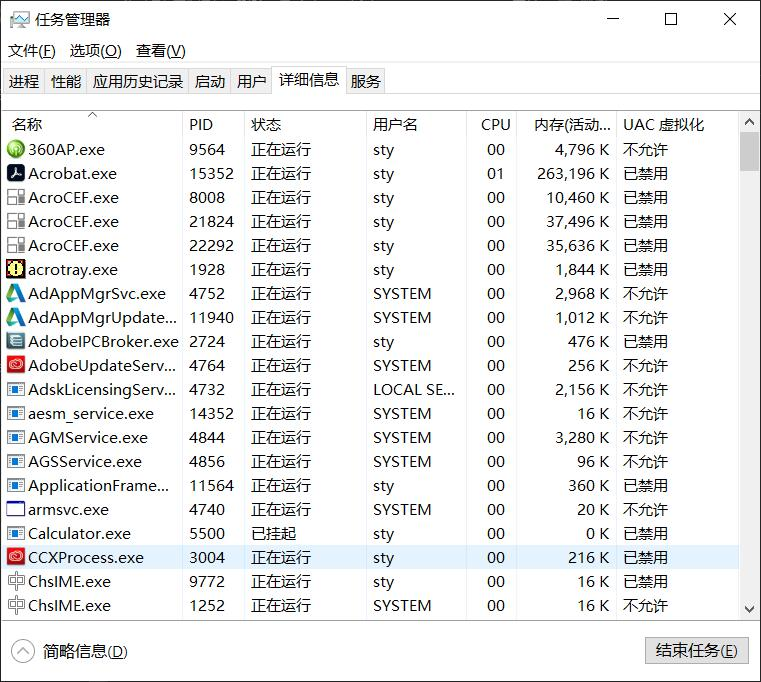
\includegraphics[width=0.7\linewidth]{screenshot001.jpg}
	\caption{进程运行状态信息}
	\label{fig:renwu}
\end{figure}
右边第一列是程序名,第二列PID列出的就是当前所有已运行程序的进程号,没有看到 命令行窗口程序(cmd)进程。

(2)	产生两个命令行窗口新进程。创建过程如图所示。

①打开两个命令行窗口。连续两次执行命令行窗口程序。
②査看命令行窗口程序的进程信息。切换到任务管理器窗口。
可以看到任务管理器窗口中新增了两行命令行程序"cmd.exe"进程信息,其进程号分别为5600和7084。

(3) 通过应用程序界面关闭进程。

1.关闭一个命令行窗口程序。
点击窗口关闭标签。

2.査看命令行窗口程序的进程信息切换到任务管理器。
可以看到进程号为5600的命令行窗口进程消失。

(4)	通过任务管理器关闭进程。
右击7084号进程-"结束进程",余下命令行窗口将被关闭,回到了原先的状态。

\subsection{实验小结}
这是一个很简单的实验,我理解了端与进程关系,了解了进程的基本概念,了解了进程的基本运行原理,掌握了基本进程管理技能。实验没有遇到困难。并且我还通过netstat -ano看到了每个进程所占用的端口号。


\section{网络端地址实验}
\subsection{实验目的}
网络端地址用于标识计算机网络进程,网络进程是计算机网络传输主体,由于语言表达上问题,容易误将计算机作为计算机网络的传输主体。明确了网络传输主体,就容易理解计算机网络各项具体功能处理的基本原理。本实验利用浏览器上网这个最为熟悉的应用,呈现网络 端地址作用。
(1)	明确计算机网络交互的主体是进程。计算机网络两台计算机之间的交互,实质上是两个进程之间的交互。
(2)	了解网络端地址构成及使用。端地址是用于标识网络上任意一台计算机上的任意一个网络进程,具有唯一性和不变性,只有通过访问网络端地址才能通过网络同该进程交互。但在日常使用应用协议时,常常忽略端口地址,自动釆用该应用协议缺省端口地址作为网络端地址。 
\subsection{实验设备}
实验环境由一台计算机来担当实验设备,计算机必须连接互联网。使用浏览器访问互联网任意一个网站,其目标网站的端地址为"www.XXX.com:80", "XXX"代表任意域名。
\subsection{实验网络拓扑}
网络端地址实验拓扑结构如图\ref{fig:screenshot001}所示。
% TODO: \usepackage{graphicx} required
\begin{figure}[htbp]
	\centering
	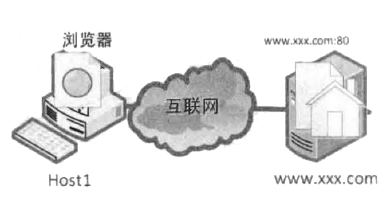
\includegraphics[width=0.7\linewidth]{image/screenshot001}
	\caption{网络端地址实验拓扑结构}
	\label{fig:screenshot001}
\end{figure}
\subsection{实验内容}
启动浏览器,通过访问同一个网址的不同端口,实验中使用了同济大学官网,实际可以是任何一个网址。

(1)	访问非80端口。地址栏中输入http://www.tongji.edu.cn:81,访问如图\ref{fig:screenshot003}所示。
% TODO: \usepackage{graphicx} required
\begin{figure}[htbp]
	\centering
	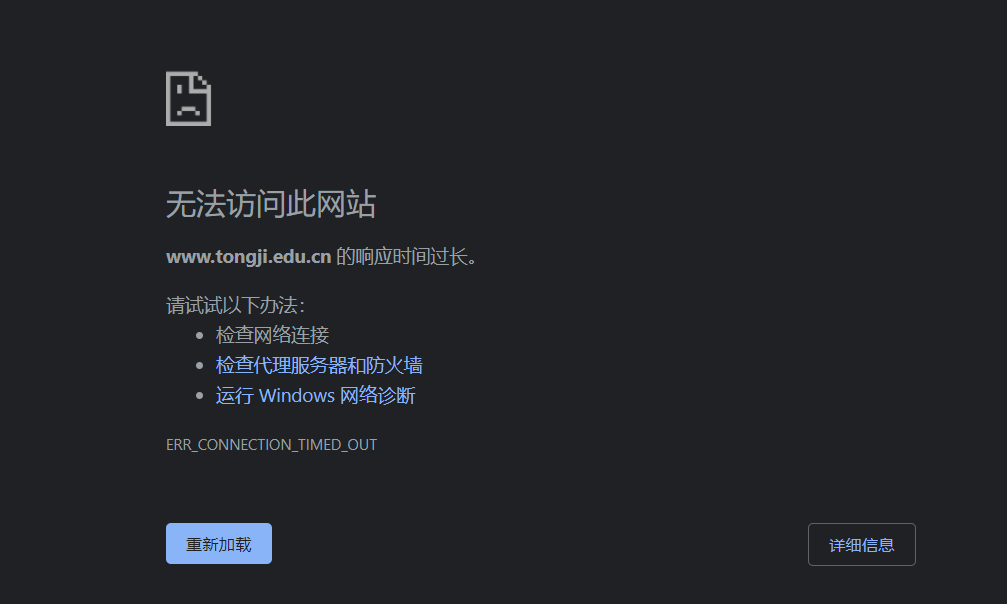
\includegraphics[width=0.7\linewidth]{image/screenshot003}
	\caption{无法访问网站}
	\label{fig:screenshot003}
\end{figure}

浏览器显示无法获得该URL地址网页,Web服务器端口地址不是81.

(2)	访问80端口,地址栏中输入"http://www.tongji.edu.cn:80",如图\ref{fig:screenshot002}所示。浏览器能正常显示网站主页内容。
% TODO: \usepackage{graphicx} required
\begin{figure}[htbp]
	\centering
	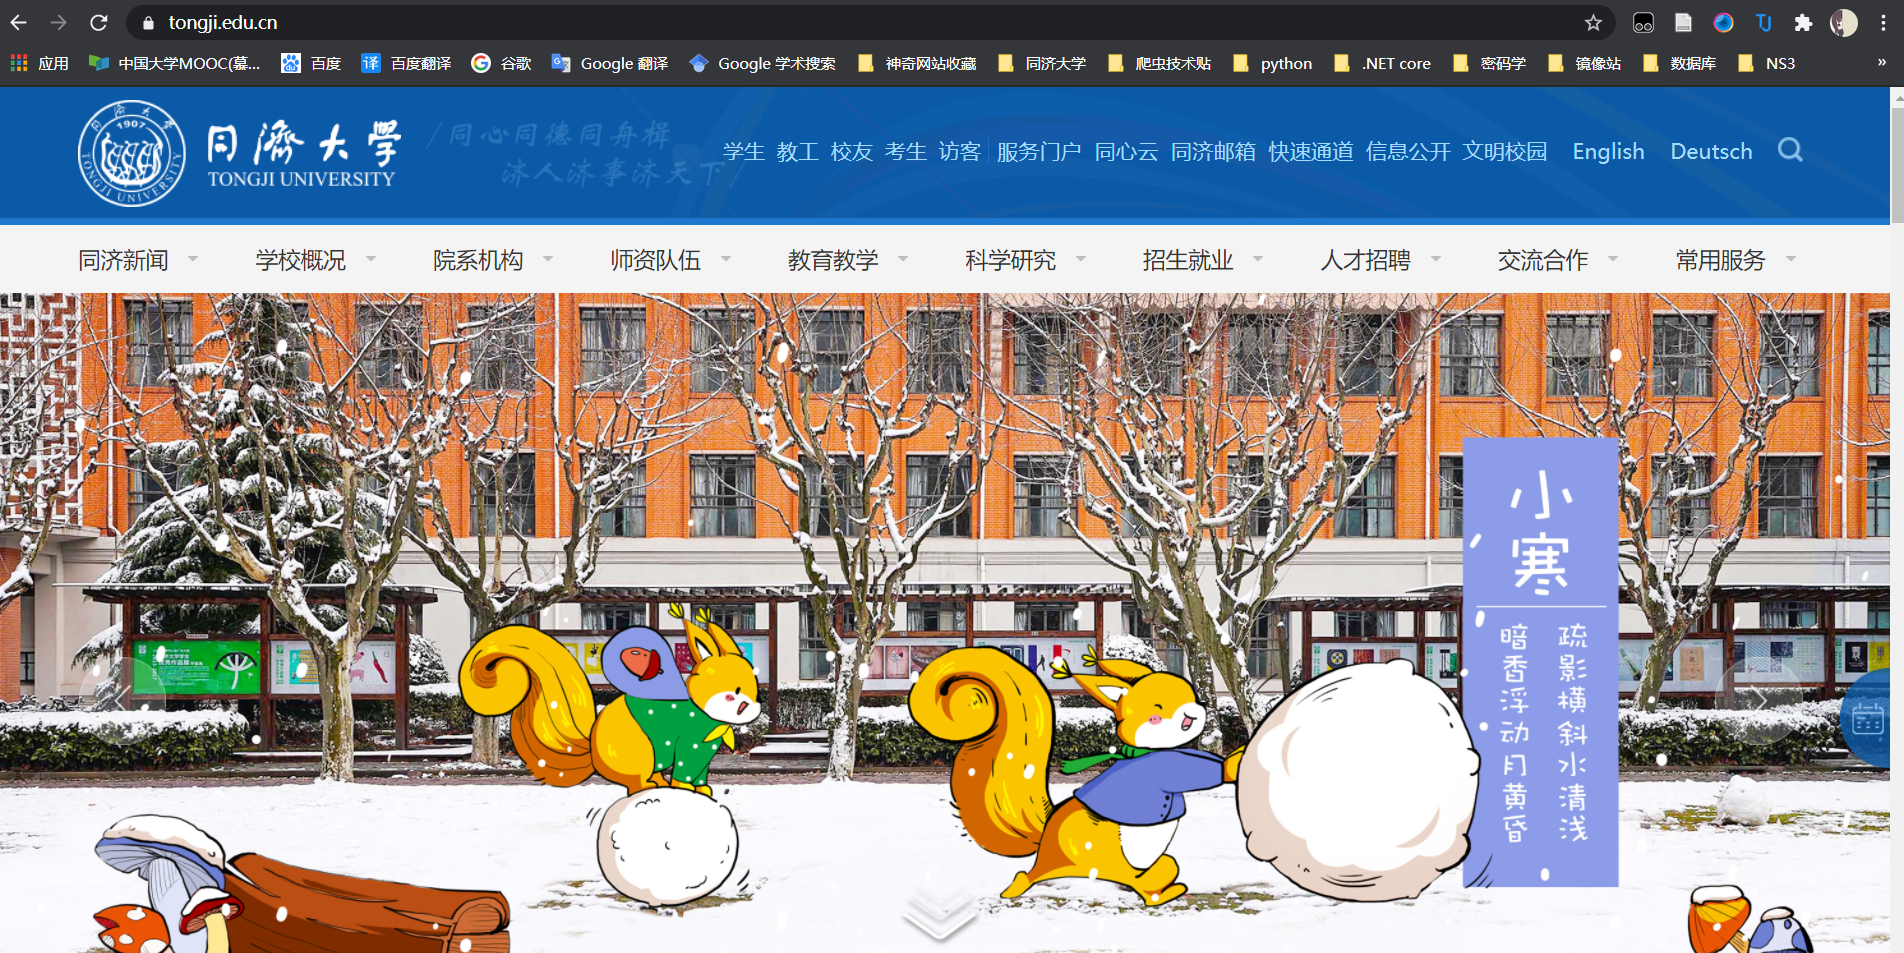
\includegraphics[width=0.7\linewidth]{image/screenshot002}
	\caption{正常访问网页}
	\label{fig:screenshot002}
\end{figure}

\subsection{实验小结}

网络端地址实验也是非常简单的实验,没有遇到任何问题。我们访问服务器的特定服务都需要指定一个特殊的端口,比如smtp协议的25端口,pop3协议的110端口,数据库使用的3306端口,https使用的443端口等等。
\section{网络线的制作和测试实验}
\subsection{实验目的}
了解以太网网络线的制作方法,深入理解物理网络的传输方式。
\subsection{实验设备}
两个TJ45水晶头,一段五类双绞线。
压线钳和网络电缆测试仪。

\subsection{实验内容}
制作一个插头,其步骤:

	1.用压线钳将网线一端的套管皮剪掉2cm。

	2.按照白橙、橙、白绿、蓝、白蓝、绿、白棕、棕线序把网线排列好。

	3.把网线摆平拉直,剪齐留下1.5cm。

	4.将水晶头有塑料弹簧片的一面向下,有金属针脚的一面向上,将线插入水晶头,并使其紧紧地顶在顶端。

	5.把水晶头插入压线钳套住水晶头用力压,使得网线和水晶头卡在一起。 

同样方法制作另一个插头

使用以太网测试工具,将网线线两端头插入网线测试仪,灯亮表示测试通过。 
\subsection{实验小结}

本次实验室我在计算机网络实验中遇到的第一个有一定难度的实验,比较考验我们的动手能力,如果没有掌握技巧,很可能在第五步"把水晶头插入压线钳套住水晶头用力压,使得网线和水晶头卡在一起"这一步失败。不过在多次尝试后,终能领略到"做网线原来如此简单"。
\section{ISO基本操作实验}
\subsection{实验目的}
1.理解实验网络物理组网原理

2.登录路由器

3.熟悉路由器操作系统ISO基本操作

\subsection{实验设备}
两台路由器,一台交换机,两台主机。

\subsection{实验网络拓扑}

% TODO: \usepackage{graphicx} required
\begin{figure}[htbp]
	\centering
	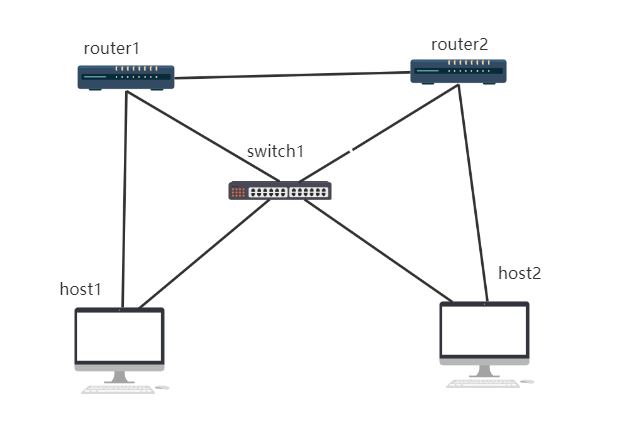
\includegraphics[width=0.7\linewidth]{image/screenshot004}
	\caption{实验网络拓扑}
	\label{fig:screenshot004}
\end{figure}

\subsection{实验内容}
\subsubsection{实验内容1}
1.观看物理连接,理解网络拓扑

2.登录路由器

--打开计算机电源

--选择系统1

--关闭防火墙

--建立HyperTerminal:开始$\rightarrow$程序$\rightarrow$附件$\rightarrow$通讯$\rightarrow$超级终端$\rightarrow$名称=router$\rightarrow$连接=com1$\rightarrow$Baut Rate=9600,8,no parity, 1 stop bit$\rightarrow$呼叫

--断开:HyperTerminal$\rightarrow$断开
\begin{table}[htbp]
	\centering
\begin{tabular}{|l|l|l|l|l|}
	\hline Command Mode & Access Method & Password & Prompt Displayed & Exit Method \\
	\hline User Exec 用户 & Log in & Virtual & $>$ & Logout \\
	\hline Privileges Exec & enable & Enable Secret & $\#$ & disable \\
	\hline Global Configuration 配早 & Config t & & (config)$\#$ & Exit/ctrl+Z \\
	\hline Interface Configuration 端口配早 & Inter & & (config-if)$\#$ & Exit/ctrl+Z \\
	\hline
\end{tabular}
\caption{ISO路由器模式}
\end{table}
\subsubsection{实验内容2}
\begin{lstlisting}
ISO基本命令
1 ?
操作帮助
--寻求帮助:router01> ?
--寻求帮助:router01> sh ?
2 show
--寻求帮助:router01> sh ?
--查看系统配置:router01> sh version
--查看路由表:router01>sh ip route
--寻求帮助:router01> sh ?
--寻求帮助:router01> sh in ?
--寻求帮助:router01> sh int g ?
--查看以太网口配置:router01> sh int gt 0/0
--寻求帮助:router01> sh int ser ?
--查看串口配置:router01> sh int serial 0/0
--查看路由表配置信息:router01> sh running-config  #权限不够
3 enable
--进入特权模式:router01>en(able) ,Enable Secret Password=cisco
--查看路由表配置信息:router01# sh running-config 
--寻求帮助:router01# sh int g ?
--查看以太网口配置:router01# sh in g 0/0
--寻求帮助:router01# sh int ser ?
--查看串口配置:router01# sh int serial 0/0
4 config
--进入配置模式:router01#config t
--寻求帮助:router01(config)# ?
5 interface
--寻求帮助:router01# inter fast ?
--进入以太口:router01(config)#int g 0/0
--修改IP地址: router01(config-if)#ip address 192.168.x.2
6 end
--退到特权模式:router01(config-if)#end(ctrl+z), exit
--查看以太网口配置:router01# sh int g 0/0
7 ping 
--连通测试命令: router01# ping 192.168.x.254
8 shut
关闭端口
--进入配置模式:router01#config t
--进入以太口:router01(config)#int g 0/0
--关闭端口功能:router01(config-if)#no shut
--退到特权模式:router01(config-if)#end(ctrl+z), exit
--查看以太网口配置:router01# sh int g 0/0
9 no
反命令
--进入配置模式:router01#config t
--进入以太口:router01(config)#int g 0/0
--打开端口功能:router01(config-if)#no shut
--退到特权模式:router01(config-if)#end(ctrl+z), exit
--查看以太网口配置:router01# sh int gt 0/0
--进入以太口:router01(config)#int g 0/0
--删除IP地址: router01(config-if)#no ip address <ipaddress><subnet mask>

\end{lstlisting}
\subsection{实验小结}
本次实验是ISO路由器基本操作试验,是后面所有实验的基础,因为后面的每次实验都需要通过命令行来操作路由器和交换机。实验内容非常简单,只需要跟着教程做就可以做出来了,本次实验了解了很多ISO操作系统的常用命令,为后面的实验打好了基础。

这段在第一次在服务器上看到的实验清单里有所以我就写了,后来又重发了个实验清单,里面没出现这个实验,因为已经写了所以就没删。

\section{UDP协议网络编程实验}
\subsection{实验目的}
UDP协议应用面没有TCP协议广,但影响也很大,如微信和QQ等都是典型的UDP应用。UDP网络编程原理基本相同。本实验是使用Socket来编写一个基于UDP简易通信程序,进行即时通信。

(1)	理解客户机/服务器模型,了解端口在网络传输中的作用。

(2)	了解无连接通信方式及编程方式。

(3)	了解掌握基于Socket的UDP应用编程的基本步骤。 

\subsection{实验设备}
一台安装了java的电脑,老师使用的IDE是Eclipse,我使用的是IDEA.
\subsection{实验内容}
运行Eclipse开发平台,并选择已创建Socket项目。

(1)	创建Java包"edu.tongji.networklab.udp"

右击项目 "MSocket/Java Resources/srcw"

"New"->"Package"

输入包名"Name=edu.tongji.networklab.udp"->"Finish"。创建该包用于存放 UDP 实验类。

(2)	开发UdpClient类。

	1.创建 UdpClient类。在包"edu.tongji.networklab.udp"下,创建 UDPClient类。 

右击"src/edu.tongji.networklab.udp"->"New"->"Class".

Name=UdpClient,选择"public static void main(String[ ] arg) "—>"Finish".

	2.输入实验代码。用附录2中UdpCIient源代码完全覆盖初始代码

	3.保存。保存包含着对Java编译,键入"Ctrl+S"或菜单"File"—>"Save"。

(3)	开发UdpServer类

	1.创建 UdpServer 类;类似 UdpCIient,在"edu.tongji.networklab.udp"下,创建 UDPServer类。 

右击"src/edu.tongji.networklab.udp"->"New"->"Class"->"Name=UdpServer",选择"public static void main(String[ ] args)"—>"Finish"

	2.代码开发。输入实验源代码,用附录2中UdpServer源代码完全覆盖初始代码。

	3.保存。保存包含着对Java编译,键入"Ctrl + S"或菜单"File"->"Save"。

(4)代码运行测试。

	1.运行UdpServerC

右击UdpServer—"Run as"->"Java Application"。

	2.运行 UdpClient 发送。同上,右击"UdpClient"->"Run as"->"Java Application"。

点击"连接",然后在发送区输入"hello"->"发送"。

	3.接收文本。
UdpClient的接收区显示"hello";左下角是UdpServer控制台,显示UdpServer收到的客户端请求数据"hello",实验成功。

下面是本次实验的截图。

% TODO: \usepackage{graphicx} required
\begin{figure}[htbp]
	\centering
	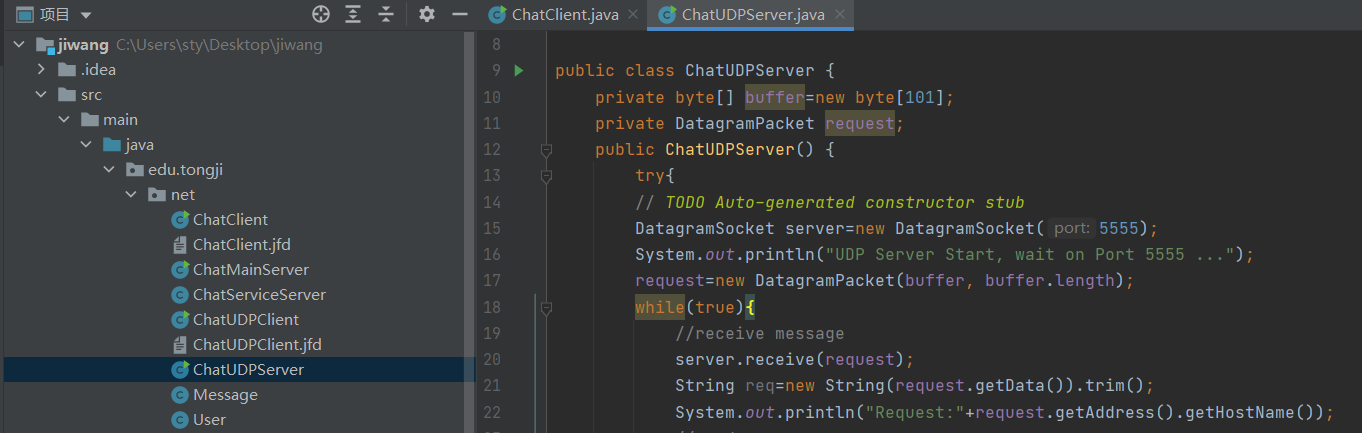
\includegraphics[width=0.9\linewidth]{image/screenshot006}
	\caption{部分代码截图}
	\label{fig:screenshot006}
\end{figure}


% TODO: \usepackage{graphicx} required
\begin{figure}[htbp]
	\centering
	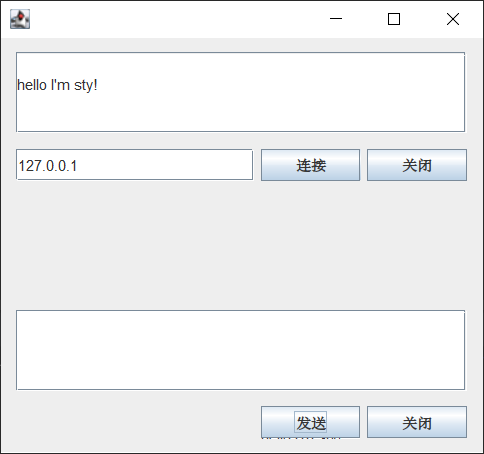
\includegraphics[width=0.7\linewidth]{image/screenshot005}
	\caption{实验截图}
	\label{fig:screenshot005}
\end{figure}


\subsection{实验小结}
实验代码金老师已经帮我们写好了,所以我们很快做完了实验,但是关键是要领会试验运行的原理,而不是只关注实验运行的结果。

这段也是在第一次在服务器上看到的实验清单里有所以我就写了,后来又重发了个实验清单,里面没出现这个实验,因为已经写了所以就也没删。

\section{TCP应用协议编程实验}
\subsection{实验目的}
TCP是使用最为广泛的传输层协议,绝大多数的网络应用服务器都使用TCP协议以保证数据传输可靠,但工程上服务器还需要具有并发能力,允许多个客户并发访问。本实验是使用Socket来编写一个基于TCP简易通信程序,且具有并发能力。
(1)	了解基于TCP网络应用服务器的基本编程架构。
(2)	了解面向连接和无连接的区别,了解TCP编程基本步骤。
(3)	了解并发服务原理及编程方式。

\subsection{实验设备}
一台安装了java的电脑,老师使用的IDE是Eclipse,我使用的是IDEA.

\subsection{实验内容}
创建实验项目目录的过程和上一个实验相似,这里不再赘述。关键点如下:

在Java项目Socket下,开发服务器程序和客户机程序。

(1)	开发服务器程序,创建并实现MainServer类和ServiceServer类,将附录3的MainServer类和ServiceServer类全部源代码复制进去。

(2)	开发客户机程序TCPClient类,为方便实验,TCPClient包含图形化界面,代码较长,将附录3的TCPClient全部源代码复制进去。

(3)	测试交互。先运行MainServer,后运行TCPClient,将连续创建两个TCPClient进程,并同时访问服务器,然后在TCPClient界面中输入字符串,测试并发通信服务。

下面是本次实验我的截图,如图\ref{fig:screenshot008} 图\ref{fig:screenshot007}:

% TODO: \usepackage{graphicx} required
\begin{figure}[htbp]
	\centering
	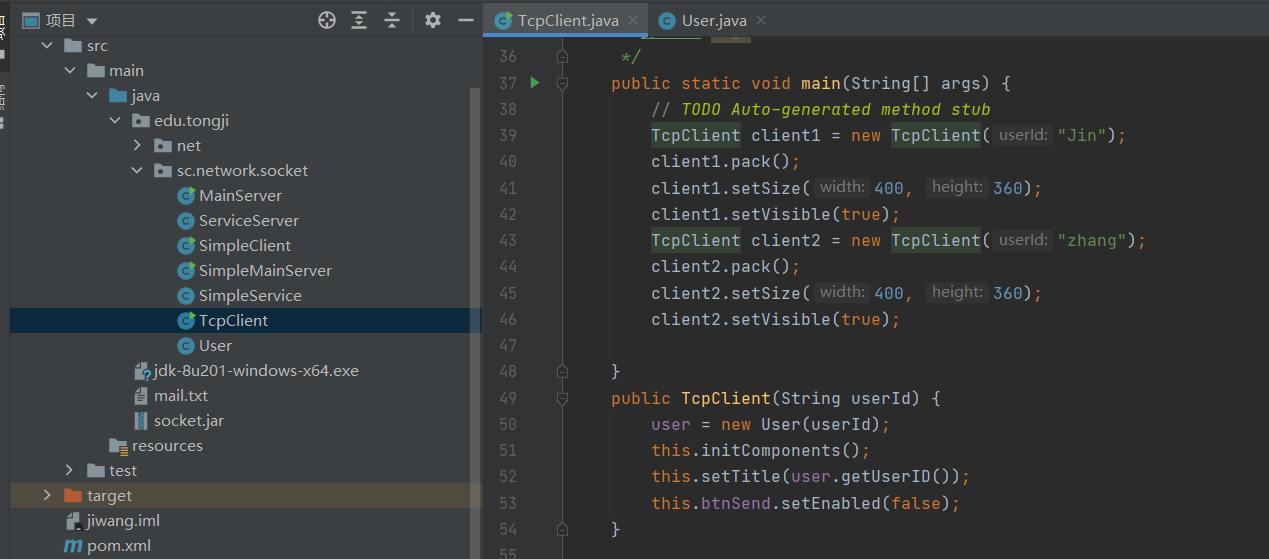
\includegraphics[width=0.8\linewidth]{image/screenshot008}
	\caption{部分代码截图}
	\label{fig:screenshot008}
\end{figure}



\begin{figure}[htbp]
	\centering
	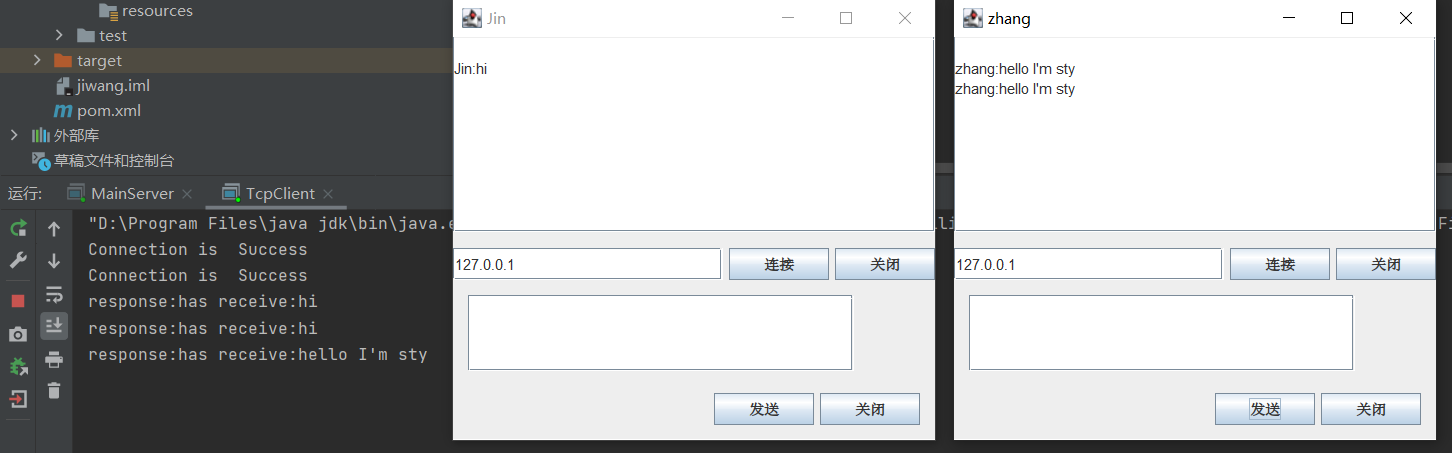
\includegraphics[width=0.8\linewidth]{image/screenshot007}
	\caption{实验截图}
	\label{fig:screenshot007}
\end{figure}


\subsection{实验小结}
这个实验和上个实验很像,TCP和UDP都是传输层协议,但具体的细节有很多很多的不同。实验代码金老师已经帮我们写好了,所以我们很快做完了实验,但是关键是要领会试验运行的原理,而不是只关注实验运行的结果。
\section{端口扫描实验}
\subsection{实验目的}
端口扫描是应对主机入侵而釆取的基本防范措施,掌握端口管理的基本技能是应对网络攻击的必备技能。本实验将使用开源的专业端口扫描软件工具nmap,对子网内的主机进行端口扫描。
(1)	了解端口开放含义。
(2)	了解安全漏洞含义。
(3)	了解掌握网络漏洞扫描工具的使用。
(4)	使用服务管理对端口进行管理。

\subsection{实验设备}

主机需要安装nmap软件。两台计算机和一台交换机担当实验设备,使用两根以太网络线,将两台计算机网卡和交换机连接起来,构成一个子网。主机Hostl作为端口扫描操作平台,另一台主机Host2作为扫描的目标平台,可以是任何一种操作系统,目标主机安装 Windows。在操作平台上使用端口扫描工具软件对目标主机进行扫描。实验使用Windows版本nmap作为端口扫描工具软件,nmap是一款开源的软件,需要下载安装。

\subsection{实验网络拓扑}


\begin{figure}[htbp]
	\centering
	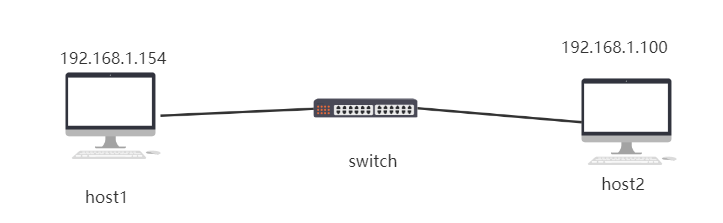
\includegraphics[width=0.7\linewidth]{image/screenshot009}
	\caption{端口扫描网络拓扑}
	\label{fig:screenshot009}
\end{figure}

\subsection{实验内容}

\subsubsection{实验一:远程子网扫描实验}

(1)	配置主机Hostl和Host2地址,主机网卡IP地址设置如下: 

Hostl:IP 地址= 192. 168.1.254,子网掩码=255.255.255.0,网关= 192.168.1.1

Host2:IP 地址= 192. 168. 1.100,子网掩码= 255.255.255.0,网关= 192.168.1.1

(2)	使用nmap扫描软件远程扫描指定子网。对192.168.1.0/24子网进行扫描。

1.Hostl 上启动 nmap。

左击“开始”->“所有程序”->“Nmap”->“Nmap-Zenmap GUI”。

2.扫描192. 168. 1.0/24子网。

输入“目标= 192. 168. 1. * ”,配置=Intense scan->“扫描”,注意扫描要持续一段时间,请保持耐心,在左边会依次列出被扫描的主机IP地址。

3.査看目标主机的端口开放状况。

选择主机192. 168. 1.100,点击“端口/主机”发现了10个开放的端口。

\subsubsection{实验二:端口关闭实验}

如果发现某些端口不用开放,就可以关闭这些端口。实验将关闭目标主机上VM认证服务端口。

(1)进入服务,关闭目标主机上VM认证服务。Host2,右击“开始”->“系统”->“其他管理工具”->“管理工具”->“服务"。

右击 VMware Anthorization Service->“停止”。

(2)重新扫描192.168.1. 100核实。由于nmap是个优秀的软件,所以只要实验网络拓扑没有断开,实验很容易就取得了成功。

实验结果如下图:

\begin{figure}[htbp]
	\centering
	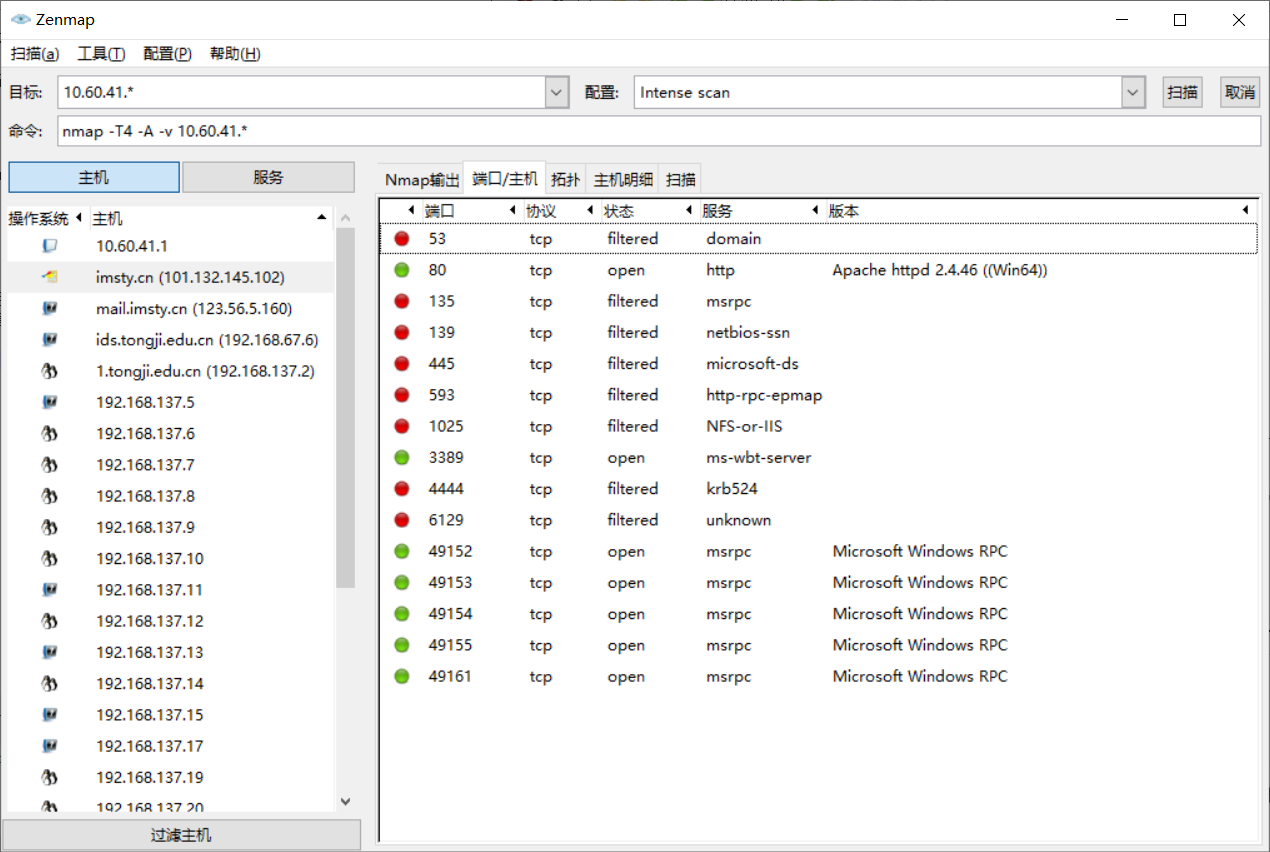
\includegraphics[width=0.7\linewidth]{image/screenshot010}
	\caption{端口扫描}
	\label{fig:screenshot010}
\end{figure}


\subsection{实验小结}
这个实验我记得其实上课金老师没带我们做,因为第一次在服务器上看到的实验清单里有所以我就写了,后来又重发了个实验清单,里面没出现这个实验,因为已经写了所以就没删。实验让我对端口扫描有了一个从感性到理性的认识,开放的网络端口确实比较容易给黑客以可乘之机,这让我想起了臭名昭著的勒索病毒WannaCry,它就是利用了Windows操作系统445端口存在的漏洞。

\section{物理地址解析实验}
\subsection{实验目的}
IP网络不具有实际通信能力,需要将IP数据包封装在物理帧中进行传输,封装前需要对下一跳IP地址进行物理地址解析。物理地址解析是理解IP封装的关键知识点,但物理地址解析行为非常隐蔽,难以察觉。实验利用ARP协议的缓存机制来间接证明物理地址解析行为的发生:
(1)	理解IP网络和物理网络之间的功能关系。
(2)	了解ARP地址解析原理。
(3)	掌握ARPT具软件使用。

\subsection{实验设备}

两台计算机和一台交换机担当实验设备,使用两根以太网络线,将两台计算机网卡都用网 线直接连接交换机。主机Hostl作为地址解析源节点,另一台主机Host2作为地址解析目标节点。使用Windows操作系统自带的ARP工具软件作为实验工具。

\subsection{实验网络拓扑}
\begin{figure}[htbp]
	\centering
	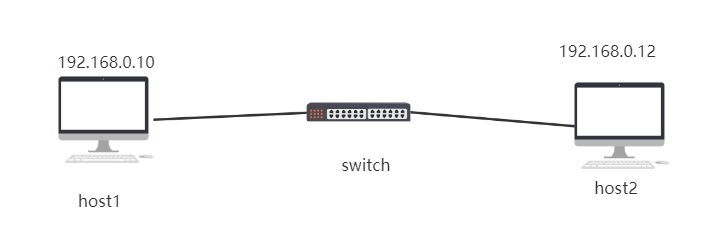
\includegraphics[width=0.7\linewidth]{image/screenshot011}
	\caption{实验网络拓扑}
	\label{fig:screenshot011}
\end{figure}


\subsection{实验内容}

按照实验环境要求,完成实验拓扑结构连接,并打开相关设备电源。

(1)	为Host1和Host2设置IP地址。主机网卡IP地址设置如下:

Host1:IP 地址= 192.168.0.12,子网掩码= 255. 255. 255.0,网关空缺

Host2:IP 地址= 192.168.0.10,子网掩码= 255. 255. 255.0,网关空缺

(2)	Host2触发对Hostl的地址解析。解析如图4-10和图4-11所示。

1.Host2清除ARP缓存表。Host2以管理员身份打开命令行窗口,清除ARP缓存表,以消除有可能存在192. 168. 0.12地址解析条目。

输入:arp-d,清空地址解析缓冲区,以便消除可能已产生的地址解析;

arp -a,显示当前地址解析缓冲区内容,没有出现192. 168.0. 12条目。

2.Host2触发对Host1地址解析,并获得其地址解析缓存。Host2发出ping连通测试命令。

输入“ping 192. 168.0. 12”,测试连通Hostl,触发对192. 168.0. 12的地址解析。

arp-a,显示当前地址解析缓存表内容,岀现了192. 168.0. 12条目,说明在发出连通测试IP数据包前,对192. 168. 0. 12节点的物理地址进行了解析,其解析物理地址是78-36-cc-ee-ab-39。

(3)	核实解析物理地址。Host1打开命令行窗口,核实物理地址。

输入“ipconfig /all”,列出IP地址和物理网卡地址,IP地址是192. 168. 0. 12,物理地址是78-36-cc-ee-ab-39,同Host2解析得到的物理地址完全一致。

实验结果如图\ref{fig:arp} 和图\ref{fig:screenshot012}所示,注意图中红框。

\begin{figure}[htbp]
	\centering
	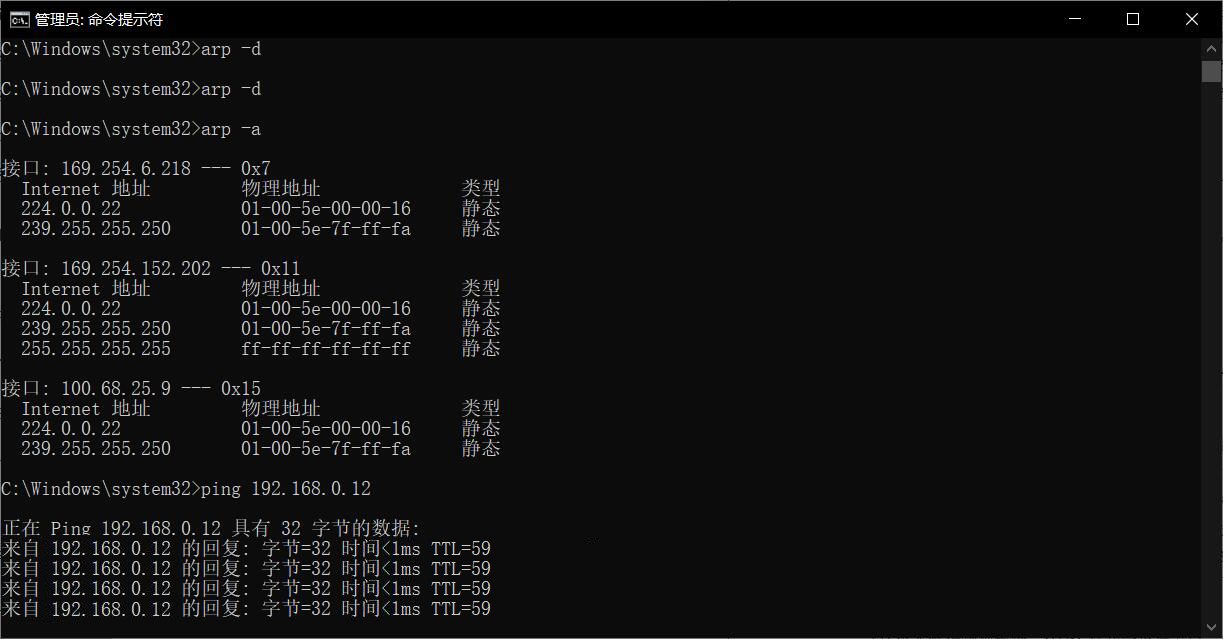
\includegraphics[width=0.7\linewidth]{arp.jpg}
	\caption{物理地址解析实验}
	\label{fig:arp}
\end{figure}


\begin{figure}[htbp]
	\centering
	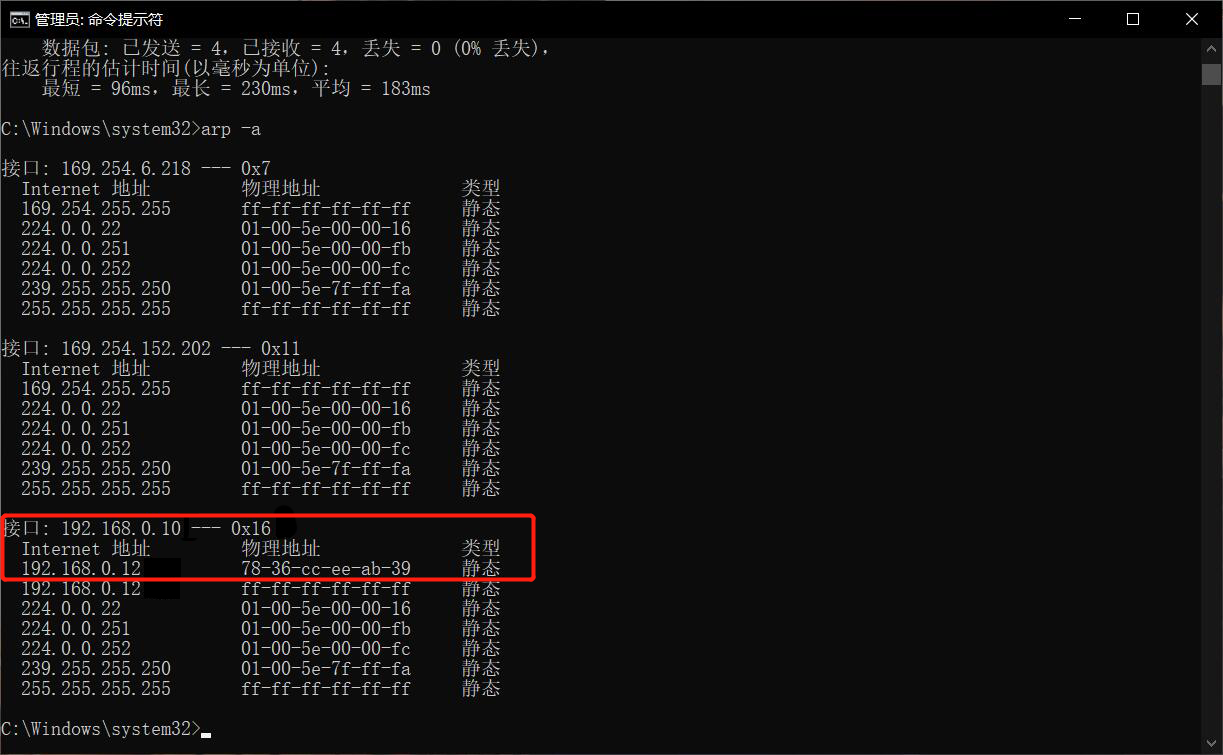
\includegraphics[width=0.7\linewidth]{image/screenshot012}
	\caption{物理地址解析实验图2}
	\label{fig:screenshot012}
\end{figure}


\subsection{实验小结}
物理地址解析实验也是非常重要的实验,实验本身没什么难度,关键在于理解。物理地址解析是通过广播ARP消息来完成的,相当于向局域网里所有主机发出一个问题:“谁拥有IP地址xxx.xxx.xxx.xxx?”然后拥有这个IP地址的主机就会回应。


\section{异步串联通信收发实验}
\subsection{实验目的}
数据通信是物理层的核心功能,其基本原理属于通信学范畴。实验利用计算机的COM口进行两台计算机间的字符收发,展示通信基本原理,加深了解物理层作用。
(1)	理解异步串行通信基本原理。
(2)	熟悉掌握RS-232通信标准以及RS-232帧格式。
(3)	了解波特率等主要通信参数的作用和使用。

\subsection{实验设备}

1. 实验环境主要由两台带COM口的计算机,1根串行交叉线组成;

2. 将单根串行交叉线中间层组成。将单根串行交叉线将两个计算机的COM串口对接起来;

3. 两台计算机超级终端将作为路由器管理的操作平台。

\subsection{实验网络拓扑}

% TODO: \usepackage{graphicx} required
\begin{figure}[htbp]
	\centering
	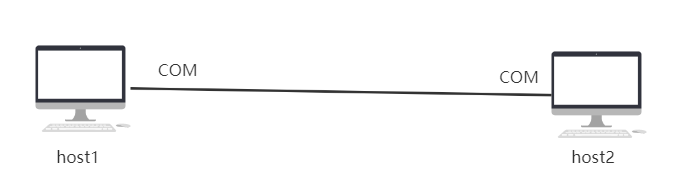
\includegraphics[width=0.7\linewidth]{image/screenshot013}
	\caption{异步串行通信试验网络拓扑}
	\label{fig:screenshot013}
\end{figure}

实验环境主要由两台带COM口的计算机,一根串行交叉线组成。将单根串行交叉线将两个计算机的COM串口对接起来;两台计算机超级终端将作为路由器管理的操作平台。

\subsection{实验内容}

【准备过程】

1. 按照实验拓扑结构要求将两台计算机的COM口用串口反接连接线连接起来。

2. Host1:运行超级终端,建立串口通信连接test1,设置缺省通信参数。

3. Host2:运行超级终端,建立串口通信连接test2,设置缺省通信参数。

\subsubsection{实验1:测试在相同通信参数下的字符传输}

1. Host2的超级终端输入如下内容,此时Host2超级终端无内容显示

\begin{lstlisting}
hello !
\end{lstlisting}

2. Host1的超级终端接收到如下字符串

\begin{lstlisting}
hello !
\end{lstlisting}

\subsubsection{实验2:测试采用不同波特率下的字符传输}

1. Host1和Host2均断开连接,在“文件->属性->配置”中修改参数如下:
\begin{table}[htbp]
	\centering
\begin{tabular}{|c|c|c|c|c|}
	\hline 连接名 & 波特率 & 数据位 & 奇偶校验 & 停止位 \\
	\hline test1 & 4800 & 8 & 奇校验 & 1 \\
	\hline test2 & 9600 & 8 & 奇校验 & 1 \\
	\hline
\end{tabular}
\caption{参数}
\end{table}

2. 进行通信测试。首先在Host1终端从键盘键入以下字符串,Host1屏幕上并不会显示输入内容,
Host2屏幕上显示乱码。

\begin{lstlisting}
7788 test
\end{lstlisting}

3. 在Host2终端从键盘键入以下字符串,Host2屏幕上并不会显示输入内容,Host1屏幕上显示不同乱
码。
\begin{lstlisting}
7788 test
\end{lstlisting}
\subsection{实验小结}

在这个实验中主要是加深我们对物理层网络通信的理性认识。实验1中,两台计算机的通信参数相同,波特率匹配,不会发生帧错误,因此字符传输正常。

而实验2中,两台计算机的波特率不同,则它们单位时间内通信信号发生变化的次数不同,相应的信号采样的频率也不一致,因此两台计算机显示出乱码且乱码值也不相同。

这个实验较简单。通过动手操作串口的字符接收和发送,加深了对通信基本原理的理解。在理解通信基本原理和异步串行传输的基础上,进一步掌握RS-232接口标准以及RS-232帧格式,通过实验1和实验2的具体操作切实理解了通信双方必须要保证波特率匹配才能正确通信,明白了波特率的物理含义。

当然实验中也遇到了一些困难,主要是串口松动接触不良造成的。
\section{主机路由实验}
\subsection{实验目的}

按照网际网组网原理,IP网络是个多跳网络,两个节点之间的传输将穿越多个IP子网,经过多个路由器,才能到达目标主机,而这一切均有赖于路由机制完成。一般认为,路由是路由器的专利。 实际上,主机上也设置了路由表,只是较为隐蔽。主机路由表是理解主机和路由器建立转发关系的 关键所在。实验构建两个IP子网,利用单路由器实现子网互联,验证主机缺省网关作用。

(1)	深入了解主机路由机制。

(2)	了解和掌握主机路由配置方法。

\subsection{实验设备}

实验环境由一台路由器、两台计算机和一台交换机组成。由交换机担当网络连接设备,将路由器两个以太网端口和两台计算机网卡都用网线直接连接到交换机;通过串行线将主机 Host1串口com同路由器Console口连接起来,启用其超级终端作为路由器管理的操作平台。

\subsection{实验网络拓扑}
主机路由实验网络拓扑如图\ref{fig:screenshot014}所示。
\begin{figure}[htbp]
	\centering
	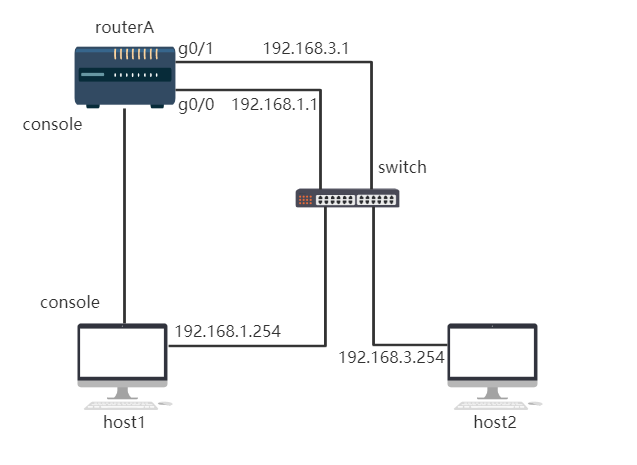
\includegraphics[width=0.7\linewidth]{image/screenshot014}
	\caption{主机路由实验网络拓扑}
	\label{fig:screenshot014}
\end{figure}


\subsection{实验内容}
按照实验环境要求,完成实验拓扑结构连接,并打开相关设备电源。

\subsubsection{实验一:主机路由实验}

(1)	配置主机Host1和Host2地址,并测试子网连通性。

1.配置Host1和Host2地址。主机网卡IP地址设置如下:

Host1: IP 地址= 192. 168. 1. 254,子网掩码= 255. 255. 255. 0,网关=192. 168. 1. 1

Host2:IP 地址= 192. 168. 3. 254,子网掩码= 255. 255. 255.0,网关= 192. 168. 3. 1

2.测试子网连通性。Host1打开命令行窗口。

输入“ping 192. 168. 3. 254”,没有连通,原因是Host1和Host2的网络地址不同,网关地址虽设置了,但网关节点并不存在,设置无法起作用。

3.查看主机Host1主机路由表。Host1使用命令行窗口。

输入"Route print",可以看到缺省路由(0.0.0.0    0.0.0.0)是 192.168. 1. 10

(2)配置RouterA以设置子网网关。启用超级终端,配置路由器两个以太网端口分别成为两个子网的网关。

\begin{lstlisting}
1. 进入配置模式。
进入特权模式:routerA>en, Enable Secret Password = cisco
进入配置模式:routerA# config t
2. 192.168.1.0/24网关配置。
进入g0/0以太网端口配置模式:routerA(config) # int g0/0
设置 IP 地址:router A (config-if) # ip address 192. 168. 1. 1 255. 255. 255. 0
开启端口:routerA( config-if) # no shut
退出端口配置模式,使端口配置生效:routerA(config-if) # exit
3. 192.168.3.0/24网关配置。
进入g0/l以太网端口配置模式:routerA(config) # in g0/l
设置 IP 地址:routerACcon£ig-if) # ip address 192. 168. 3. 1 255. 255. 255. 0
开启端口:routerA( config-if) # no shut
退出端口配置模式,使端口配置生效:routerA(config-if) # exit
4. 启用路由功能。
启用路由功能:routerA(config) # ip routing
退出配置模式,使配置生效:routerACconfig) # exit

\end{lstlisting}

(3)	测试子网连通性。测试主机Host1是否连通主机Host2, Host1中打开命令行窗口,输入"ping 192. 168. 3. 254”,表示Host1已连通主机Host2,主机路由表和主机网关发生作用,发挥了路由器路由转发功能。

\subsubsection{实验二:主机缺省网关实验}

取消主机Host1缺省网关地址,并测试同Host2连通性。

(1)	重置主机Hostl的缺省网关地址。

删除默认网关地址-“确定”。

(2)	测试子网连通性。Hostl打开命令行窗口。

输入“ping 192.168.3.254”,表示不能连通Host2,网关节点存在,但主机的网关地址没有设置,将不能发挥网关节点作用,无法访问其他子网。


\subsection{实验小结}

在实验过程中出现了一些问题,例如接上交换机并配置完每台主机的IP和子网掩码后,利用ping进行连通性测试失败,后经检查后发现网线刚接上交换机时交换机对应端口的灯为红色,等待灯变成绿色后可以成功ping通,猜测是因为此段时间交换机在获取主机的IP地址或者MAC地址。

在实验时,用网线将路由器的FE 0/1口和FE 0/0口和交换机相连,路由器和交换机对应端口的灯亮,但是过一会之后路由器上的FE 0/1端口灯灭了,对应的交换机端口上的灯也灭了,我以为是路由器坏了,后来发现,在对路由器进行操作,输入no shut命令开启FE 0/1端口之后灯又亮了,由此我明白了为什么开启端口的命令叫做no shut。在对路由器进行操作的时候碰到的另一个问题是,我根据书上的命令进行输入,输入int g0/0回车,命令行报错,经过排查之后发现我使用的路由器上的端口名称不是g0/0而是 FE 0/0,这可能是因为路由器不是千兆路由器而是百兆路由器,因此我将命令改成了int f0/0,遂成功。

在实验中还遇到了另外的问题是,所有操作均正确,但是主机却ping不通,根据老师的点拨,是因为交换机可能已经划分了多个VLAN,因此更换接线的端口之后成功ping通。
\section{以太网组网实验}
\subsection{实验目的}

物理网络是计算机网络的基本组织单元,其各个节点之间可以进行数据通信。物理网络是互联网的基础架构,无论对于理解网络基本原理还是网际互联原理都非常关键。实验利用以太网交换机组成一个独立的双绞线以太网物理网络,实现网络节点之间的互通。

(1)	理解局域网组网原理。

(2)	理解掌握以太网组网步骤。

(3)	了解以太网网络地址格式。

\subsection{实验设备}

两台计算机和一台交换机担当实验设备,使用两根双绞线网线,将两台计算机以太网网卡同交换机连接起来。计算机Host1作为操作平台和测试操作平台,另一台计算机Host2作为测试平台。也可以使用家用无线路由器代替交换机,开展本实验。

\subsection{实验网络拓扑}

如图\ref{fig:screenshot015}所示

\begin{figure}[htbp]
	\centering
	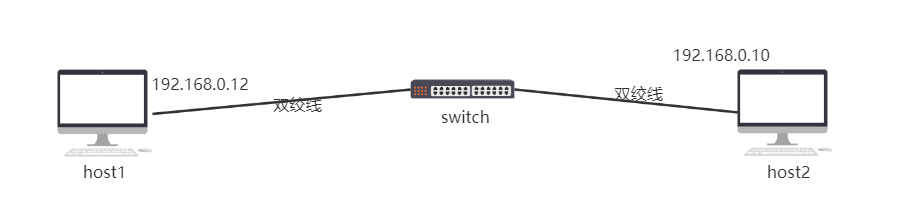
\includegraphics[width=0.7\linewidth]{image/screenshot015}
	\caption{组网实验实验网络拓扑图}
	\label{fig:screenshot015}
\end{figure}

\subsection{实验内容}

\subsubsection{实验一:以太网组网试验}

(1)	用两根双绞线网线分别将两台计算机网卡同交换机端口连接起来,这样就形成了局域网。

(2)	为主机配置IP地址。限于篇幅,请参考1.4. 1小节,主机网卡IP地址设置如下。

Hostl:IP 地址= 192. 168. 0. 12,子网掩码= 255. 255. 255.0

Host2:IP 地址= 192. 168. 0. 10,子网掩码= 255. 255. 255. 0

(3)	Host1测试Host2是否连通。打开Host1命令行窗口。

输入ping命令“ping 192. 168.0. 10”,可以看到连通,由于交换机处理有个延缓过程,命令要多打几次,才能实验成功。

这个地方我印象深刻,交换机上的灯过一会之后会由红变绿,代表可以连通了。

实验截图如下:

% TODO: \usepackage{graphicx} required
\begin{figure}[htbp]
	\centering
	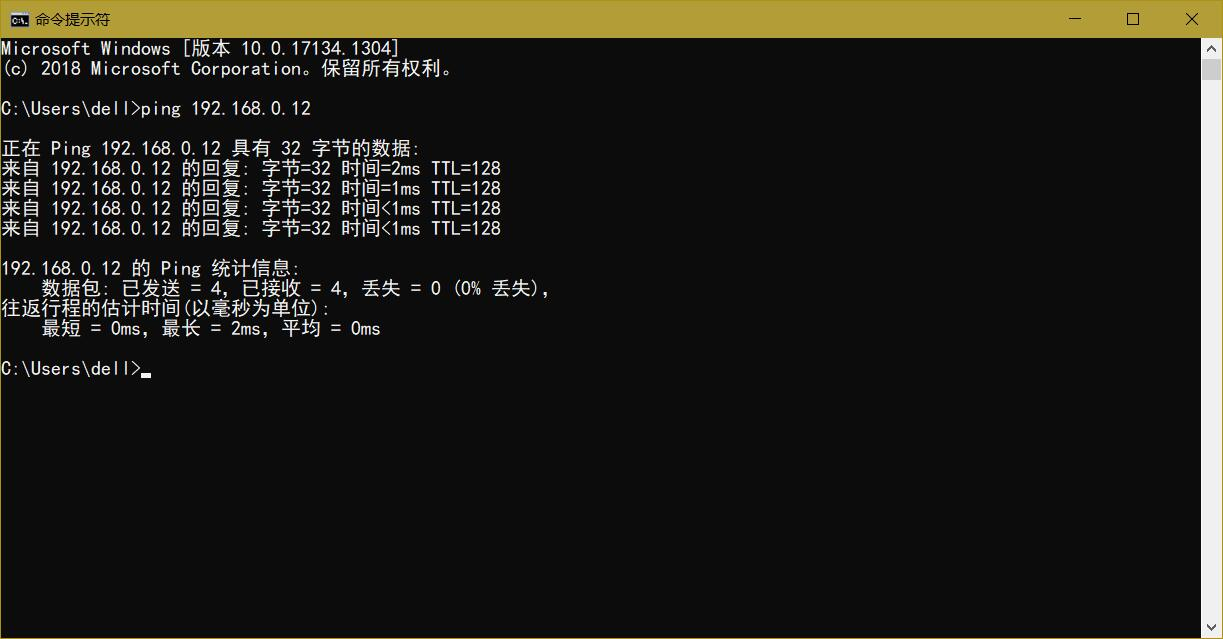
\includegraphics[width=0.7\linewidth]{image/ping}
	\caption{ping通了}
	\label{fig:ping}
\end{figure}



\subsubsection{实验二:以太网卡地址查看实验}

Host1査看自身以太网物理地址,打开命令行窗口。

输入命令ipconfig: ipconfig /all,可以看到Host1以太网卡的IP地址和物理地址。

% TODO: \usepackage{graphicx} required
\begin{figure}[htbp]
	\centering
	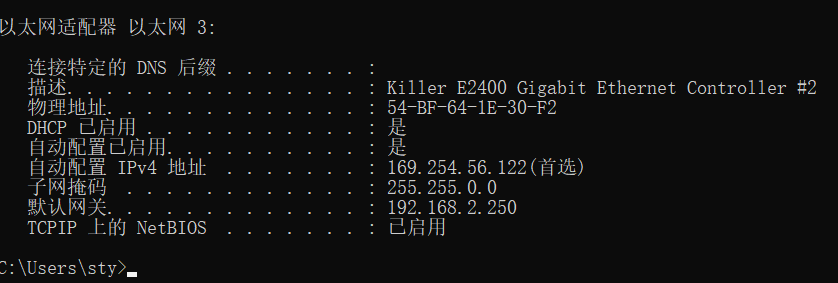
\includegraphics[width=0.7\linewidth]{image/screenshot016}
	\caption{查看地址}
	\label{fig:screenshot016}
\end{figure}


\subsection{实验小结}

这两个实验的内容相当相当的简单,但在当时做实验的时候还是遇到了一点点小问题,例如接上交换机并配置完每台主机的IP和子网掩码后,利用ping进行连通性测试失败,后经检查后发现网线刚接上交换机时交换机对应端口的灯为红色,等待灯变成绿色后可以成功ping通,猜测是因为此段时间交换机在获取主机的IP地址或者MAC地址。

在实验中还遇到了另外的问题是,所有操作均正确,但是主机却ping不通,根据老师的点拨,是因为交换机可能已经划分了多个VLAN,因此更换接线的端口之后成功ping通。

\section{VLAN配置实验}
\subsection{实验目的}

对于企业而言,可能含有许多部门,为便于管理,常常以部门为单位,构建多个物理子网。 传统网络工程,只有相近的办公室才可以组成同一个物理子网,鉴于种种原因,很可能同个部 门的两个办公室位于不同楼层,甚至不同大楼。

虚拟局域网(Virtual Local Area Network, VLAN),标准编号为IEEE 802.IQ,可以实现 将两个相距较远的办公室组成同一个物理子网。实验利用交换机提供虚拟局域网功能,实现VLAN划分。

(1)	了解虚拟局域网基本概念。

(2)	掌握交换机实施虚拟局域网技术。


\subsection{实验设备}

由一台CISCO交换机和两台计算机担当实验设 备,使用两根双绞线网线,将两台计算机以太网网卡同交换机连接起来;通过串行线将计算机Hostl串口 coml同交换机Console 口连接起来,使用超级终端作为交换机的操作平台。


\subsection{实验网络拓扑}

如图,我将不同的端口区分了不同的颜色以区分它们,代表不同的VLAN.

\begin{figure}[htbp]
	\centering
	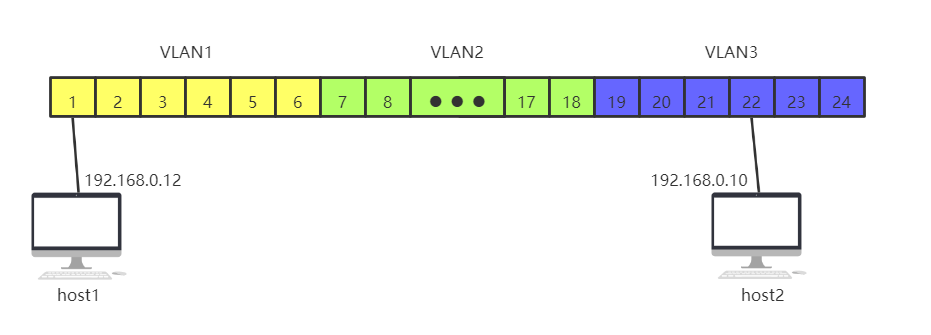
\includegraphics[width=0.7\linewidth]{image/screenshot017}
	\caption{VLAN划分示意图}
	\label{fig:screenshot017}
\end{figure}


\subsection{实验内容}

\begin{lstlisting}
1.未配置前端口通信测试
--配置两主机IP地址:192.168.0.2和192.168.0.5
--连接任意端口
--测试192.168.0.2:ping 192.168.0.5#连通
2配置VLAN2
2.1连接交换机
--使用console线将计算机串口com2与路由器console口直接相连;
--建立HyperTerminal:开始程序附件通讯超级终端名称=switch连接=com2Baut Rate=9600,8,no parity, 1 stop bit;
--进入特权模式:switch01>en(able) ,Enable Secret Password=cisco
2.2 2查看VLAN配置:switch01# sh vlan
2.2.3 建立VLAN2
--进入vlan配置模式:switch01#vlan database
--添加vlan: switch01(vlan)#vlan 2 name vlan2 
--退出:switch01(vlan)#exit
2.2.3 建立VLAN3
--进入vlan配置模式:switch01#vlan database
--添加vlan: switch01(vlan)#vlan 3 name myvlan 
--退出:switch01(vlan)#exit
2.2.4 为VLAN2分配端口
--进入配置模式:switch01#config t
--进入f0/1端口:switch01(config)#in f0/1
--将端口分配给vlan2:switch01(config -if)#switchport access vlan 2
--退出:switch01(config -if)#exit
--查看VLAN2配置:switch01# sh vlan name vlan2
2.2.5.测试
--重新测试192.168.0.2: ping 192.168.0.5 #不连通
2.2.6 为VLAN2分配新端口
--进入f0/24端口:switch01(config)#in f0/24
--将端口分配给vlan2:switch01(config -if)#switchport access vlan 2
--退出:switch01(config -if)#exit
--查看VLAN2配置:switch01# sh vlan name vlan2
2.2.7.测试
--重新测试192.168.0.2: ping 192.168.0.5 #办连通
3配置VLAN3
4 删除VLAN
4.1 删除端口
--进入配置模式:switch01#config t
--进入f0/1端口:switch01(config)#in f0/1
--将端口返回VLAN1:switch01(config -if)#switchport access vlan 1
--将所有端口删除
--退出:switch01(config -if)#exit
4.2 删除VLAN2
--进入vlan配置模式:switch01#vlan database
--添加vlan: switch01(vlan)#no vlan 2
--退出:switch01(vlan)#exit
4.3查看VLAN配置:switch01# sh vlan
4.4 删除VLAN3
--进入vlan配置模式:switch01#vlan database
--添加vlan: switch01(vlan)#no vlan 3
--退出:switch01(vlan)#exit

\end{lstlisting}

实验过程的记录如下,每幅图的含义已经写在每幅图片的下方:


\begin{figure}[htbp]
	\centering
	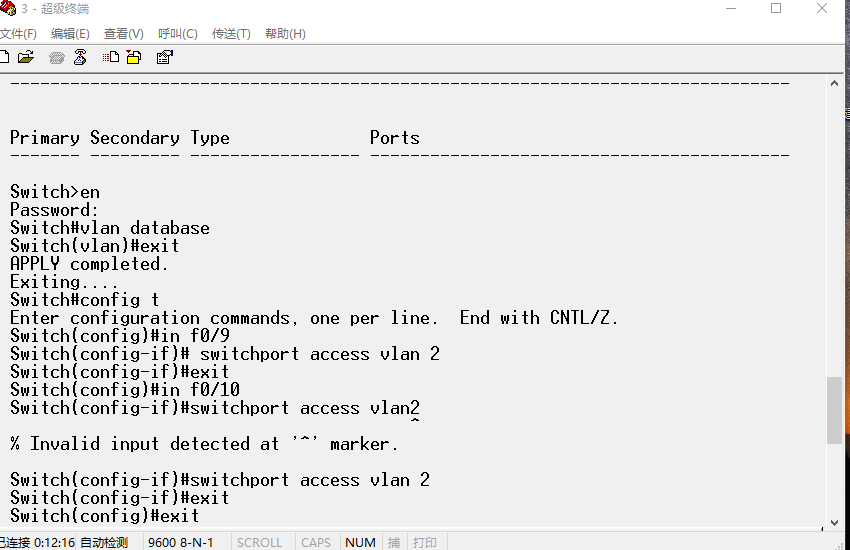
\includegraphics[width=0.7\linewidth]{image/vlan1}
	\caption{为端口指定VLAN}
	\label{fig:vlan1}
\end{figure}

\begin{figure}[htbp]
	\centering
	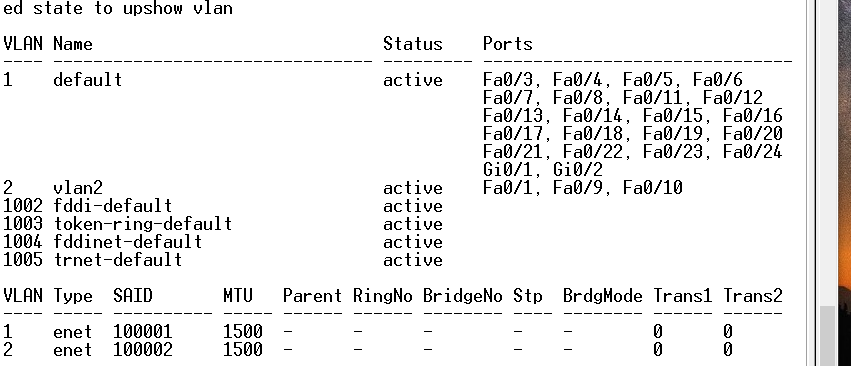
\includegraphics[width=0.7\linewidth]{image/vlan2}
	\caption{查看已经划分的端口}
	\label{fig:vlan2}
\end{figure}

\begin{figure}[htbp]
	\centering
	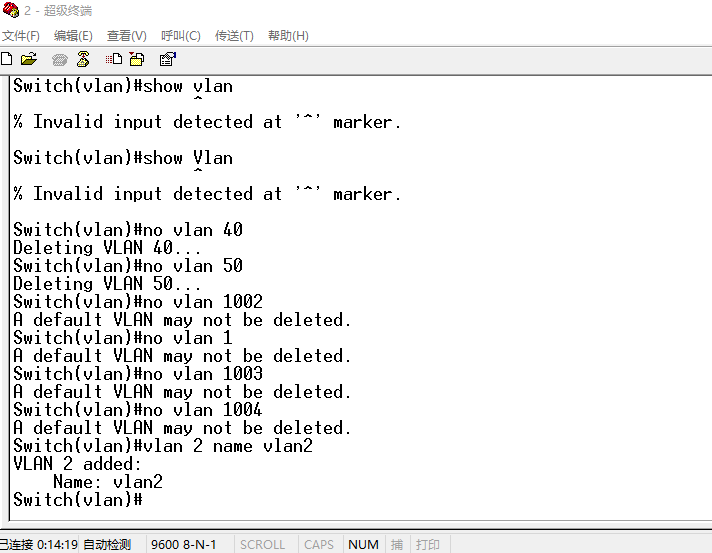
\includegraphics[width=0.7\linewidth]{image/vlan3}
	\caption{删除VLAN以及添加VLAN}
	\label{fig:vlan3}
\end{figure}


\begin{figure}[htbp]
	\centering
	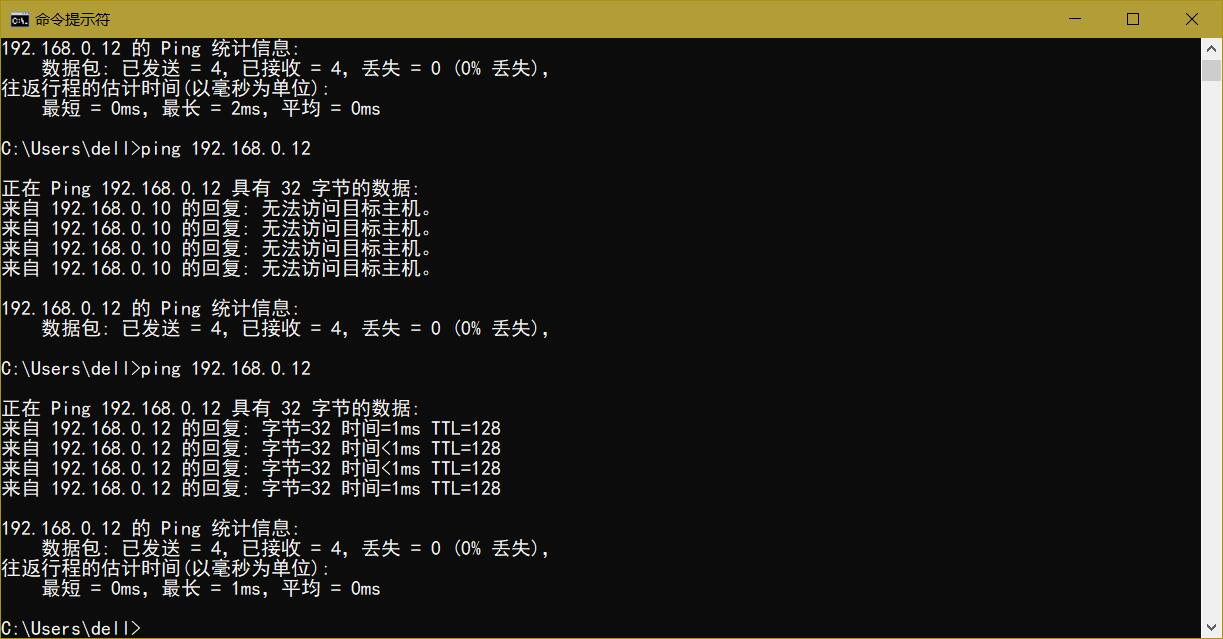
\includegraphics[width=0.7\linewidth]{image/在不同vlan无法访问,在相同vlan可以访问}
	\caption{在不同vlan无法访问,在相同vlan可以访问}
	\label{fig:vlanvlan}
\end{figure}



\subsection{实验小结}

VLAN实验可以算是非常实用的实验了,因为为了局域网的安全,给网络划分不同的区域非常重要。计网实验指定很多,使用也比较复杂,必须静下心来仔细核对,否则就比较容易出错。另外实验室的设备也有时候会出一点问题导致实验进度受到阻碍。

尚未配置VLAN前,VLAN1拥有所有端口,1个VLAN即1个广播域,在同广播域下的192.168.0.10与192.168.0.12可以连通。但如果在不同的VLAN中就无法连通了。

\subsubsection{经验教训}

配置完之后检查一下VLAN分配情况看看是不是你想的那样,而且前面的同学留下来的配置也可能干扰你做实验。

\section{虚拟无线网络实验}
\subsection{实验目的}

无线组网技术是计算机网络组网技术中发展最为迅速的技术,由于无线网络具有的可移动性,发展前景非常广阔,但无线组网技术实验教学却受环境制约因素较大,无论设备数量还是拓扑结构,在现有实验条件下均受到极大限制。

在经过本实验之后,可以对NS3这一平台有更深入的理解。


\subsection{实验设备}
一台安装了VMware的电脑,其中安装Ubuntu 16.04,并配置好NS3的环境。

\subsection{实验内容}

本实验包括两个部分。

\subsubsection{1.无线局域网络隐藏节点实验}

【实验目标】

对无线网络的传输机制有一个直观的了解,加深对CSMA/CA协议的理解。该实验项目中可以随意调整节点的位置,并通过分析实验产生数据结果,来获得最终的实验结论。可以培养初步的观察力和分析能力,形成最基本的研究能力。

【实验原理】

无线局域网络Wireless LANs,简称Wi-Fi,标准版本号是802.11,从此版本又发展了多个子版本,比如熟知的802.11g。但其传输机制是完全一致,所有节点都采用了同频率载波,采用了Carrier Sense On Multi-Access/ Collision Avoid (CSMA/CA),即多路存取载波监听/避免碰撞机制,类似总线的共享发送模式,即任意时刻只有一个节点才能发送。
多路存取载波监听机制,根据监听通道传输状态以决定是否可以发送。

1、当节点需要发送数据时,进行载波监听。载波是网络上的传输信号。

2、如果节点在网络上监听到载波,说明其他节点在发送,那只能耐心等待,返回1。

3、如果没有监听到载波,就能直接往网上发送帧,用不着通知其他节点。这是没有节点在传输数据。

多路存取载波监听机制建立在所有节点都能监听其他任意节点的载波基础上,但在无线网络中,由于其可移动性,会发生隐藏节点问题。

隐藏节点是指在接收节点的覆盖范围内而在发送节点的覆盖范围外的节点。由于听不到发送节点的发送,隐藏节点可能向相同的接收节点发送分组,导致分组在接收节点处冲突。隐藏节点可以分为隐发送节点和隐接收节点。

A和C就互为隐藏节点。节点A和C同时想发送数据给节点B,但A和C都不在对方的传送范围内。所以当A发送数据给B时,C并未检测到A也在发送数据,会认为目前网络中无数据传送,会将数据发送给B。这样,A和C同时将数据发送给B,使得数据在B处产生冲突,最终导致发送的数据不可用。这种因传送距离而发生误判的问题称为隐藏节点问题。

解决隐藏节点的思路是使接收节点周围的邻居节点都能了解到正在进行的传输。RTS/CTS方式是解决隐藏节点问题的主要方法之一,发送节点在数据发送前与接收节点进行一次短控制消息握手交换,请求发送(Request to Send,RTS)和清除发送(Clear to Send,CTS)的控制信息来避免冲突。

发送方发出数据前,先送出一个RTS包,告知在传送范围内的所有节点不要有任何传送操作。如果接收方目前空闲,则响应一个CTS包,告诉发送方可开始发送数据,此CTS包就会告知所有在接收方信号传输范围内的其它节点不要进行任何传输操作。

【实验内容】

隐藏节点实验主要是揭示无线节点传输过程中可能发生的冲突以及解决的过程。实验设置了两个发送节点和一个接收节点,实验中需要控制的是节点之间的距离可以自由调整,RTS/CTS控制可以启用或不启用,然后观察数据包丢失现象来获得实验结论。实验场景如下:

\begin{figure}[htbp]
	\centering
	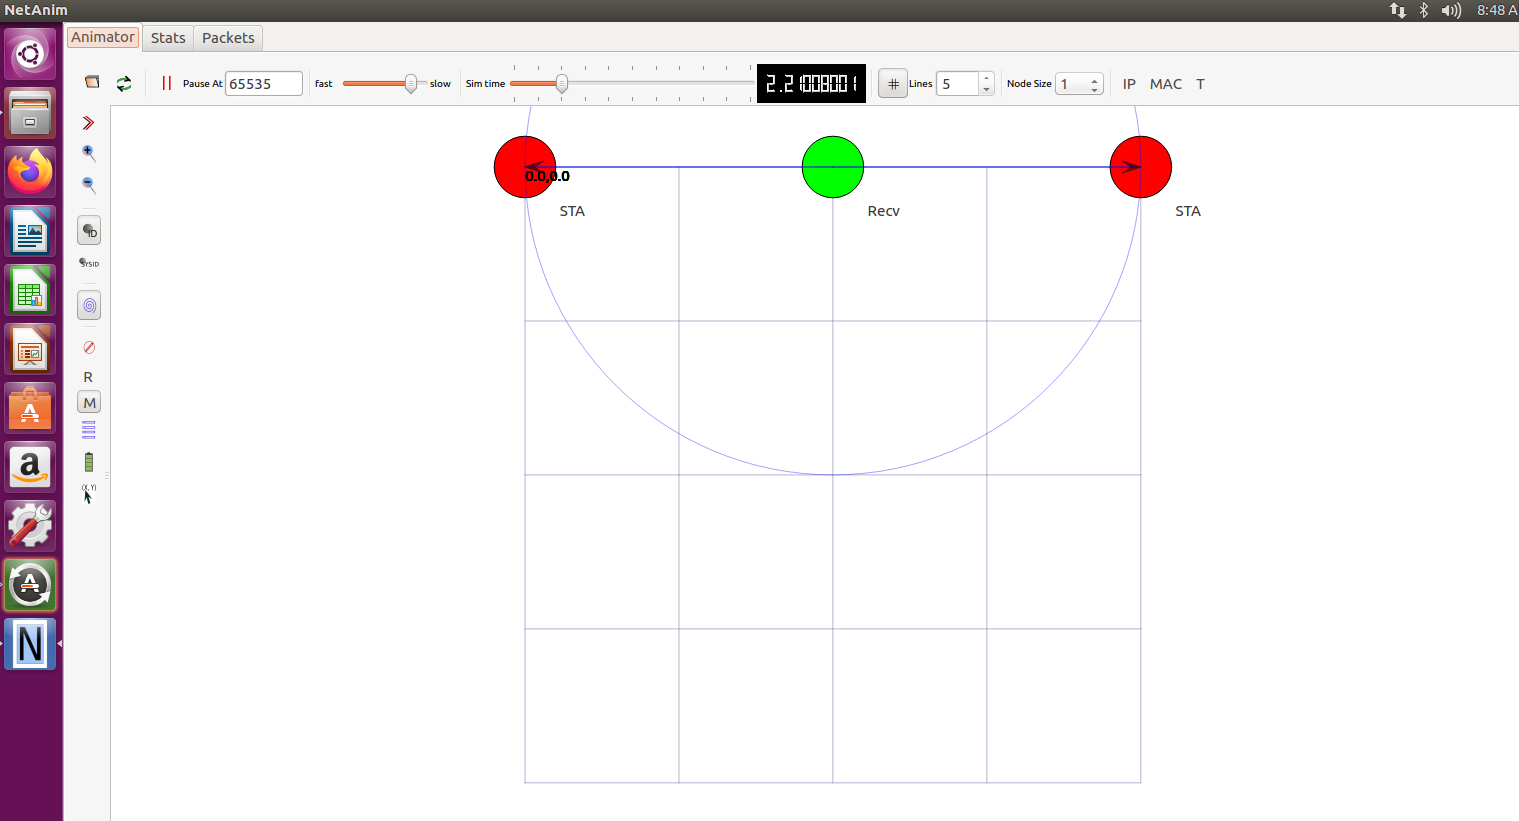
\includegraphics[width=0.7\linewidth]{image/screenshot019}
	\caption{实验场景}
	\label{fig:screenshot019}
\end{figure}

【实验过程】

虚拟实验由wifi-hidden-stations.cc实现。具体步骤:

1、编译wifi-hidden-stations.cc。

1)复制wifi-hidden-stations.cc到NS\_HOME/scratch

2)编译wifi-hidden-stations.cc:./waf –run scratch/wifi-hidden-stations.cc

\begin{figure}[htbp]
	\centering
	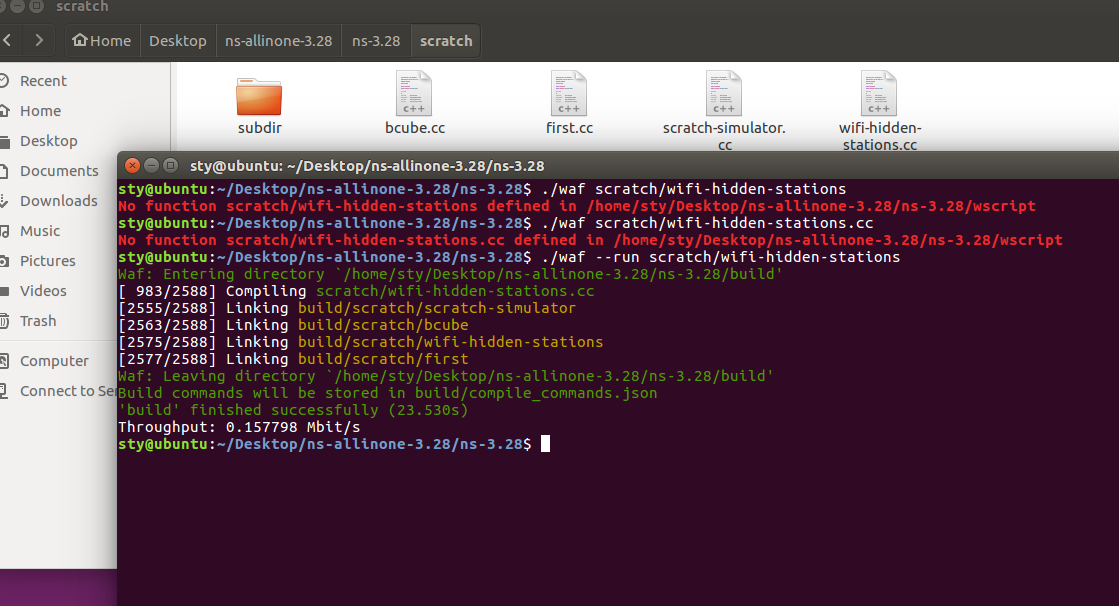
\includegraphics[width=0.9\linewidth]{image/screenshot018}
	\caption{编译并运行wifi-hidden-stations.cc}
	\label{fig:screenshot018}
\end{figure}

2、运行目标代码。

1)将目录移动到NS\_HOME/scratch/build

2)运行目标代码:./ wifi-hidden-stations.cc

3、显示运行动画

1)将目录移动到执行目录netanim

2)启动netanim动画工具程序:./NetAnim

3)显示运行动画。打开wifi-hidden-stations.xml


\begin{figure}[htbp]
	\centering
	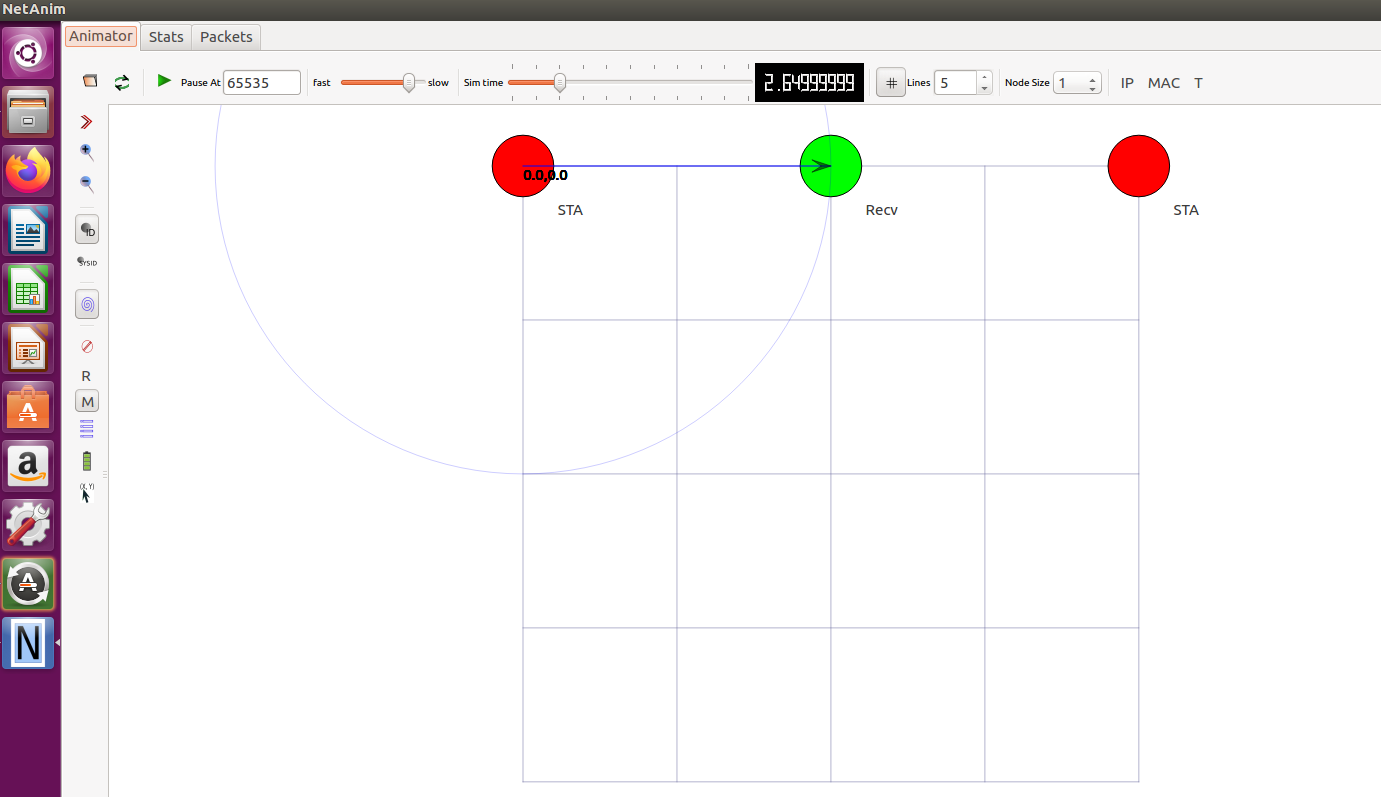
\includegraphics[width=0.9\linewidth]{image/screenshot020}
	\caption{运行画面}
	\label{fig:screenshot020}
\end{figure}

【实验小结】

通过本次实验以及源码阅读我初步知道了如何编写一个ns3脚本来模拟一个预设的网络场景,掌握了科学研究的工具是进行科学研究的第一步。

隐藏节点的问题是计算机网络中经常被拿来讨论的问题,可是只有亲自写过代码清楚其中的逻辑才能完全掌握它。

\subsubsection{2.移动自组网络manet实验}

【实验目标】

实验目标,主要是对移动自组网络的传输机制有一个直观的了解,加深对中间节点路由协议原理的理解,培养学生的初步的观察力和分析能力,形成最基本的研究能力。

【实验原理】

自组网络实验主要是揭示其典型的传输过程。工程上,经常将数据发送节点,称为源(source)节点,主要用于采集数据,接收节点,称为汇聚(sink)节点,将收集到的数据统一发送给数据中心。实验将使用50个节点,其位置随机确定的,其中,确定1个汇聚节点和10个源节点,源节点将同时向汇聚节点发送数据,不能直接传输到达的数据,将由其他中间节点进行路由,实验允许采用OLSR、AODV、DSDV和DSR路由协议,缺省采用AODV路由协议。通过观察数据包传输来理解自组网络运行机制。

AODV无线自组织按需距离矢量协议. 当一个节点需要给网络中的其他节点传送信息时,如果没有到达目标节点的路由,则必须先以组播的形式发出RREQ(路由请求)报文。RREQ报文中记录着发起节点和目标节点的网络层地址,邻近节点收到RREQ,首先判断目标节点是否为自己。如果是,则向发起节点发送RREP(路由回应);如果不是,则首先在路由表中查找是否有到达目标节点的路由,如果有,则向源节点单播RREP,否则继续转发RREQ进行查找。


\begin{figure}[htbp]
	\centering
	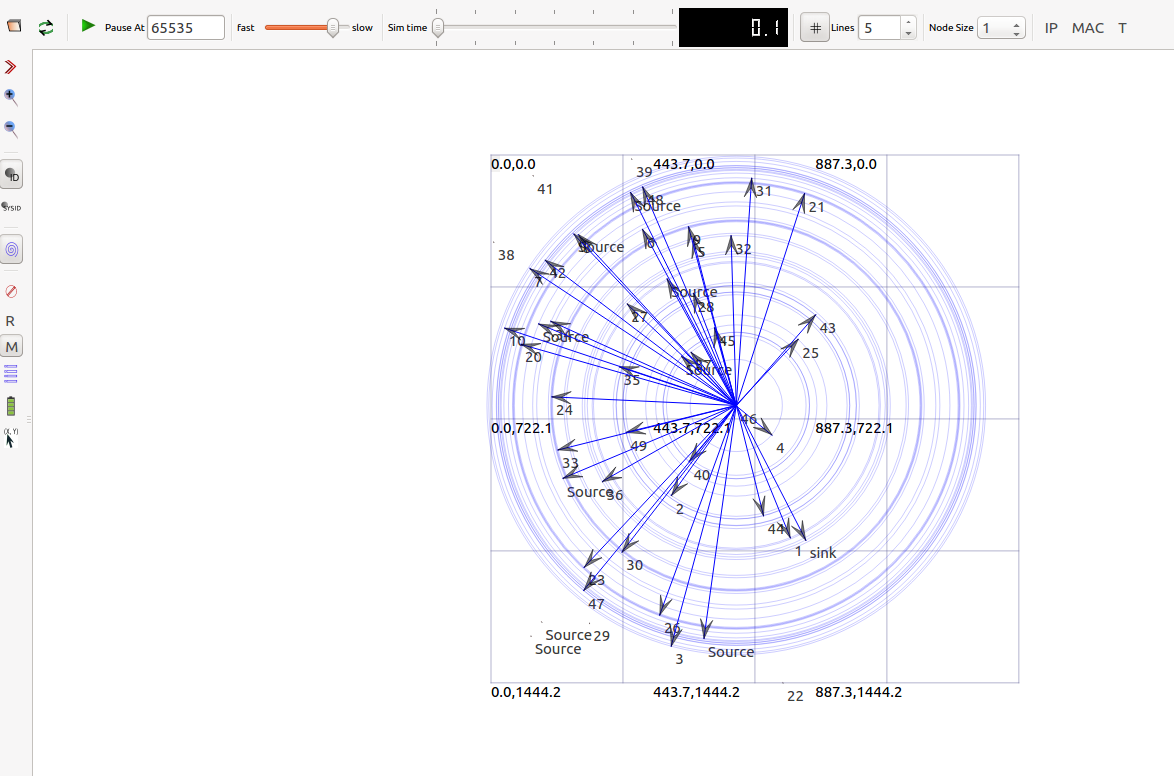
\includegraphics[width=0.8\linewidth]{image/screenshot023}
	\caption{实验界面示意}
	\label{fig:screenshot023}
\end{figure}



【实验内容】

虚拟实验由manet-routing.cc实现。具体步骤:

1、编译manet-routing..cc。

1)复制manet-routing.cc到NS\_HOME/scratch

2)编译manet-routing.cc:./waf –run scratch/ manet-routing.cc

2、运行目标代码。

1)将目录移动到NS\_HOME/scratch/build

2)运行目标代码:./ manet-routing.cc

\begin{figure}[htbp]
	\centering
	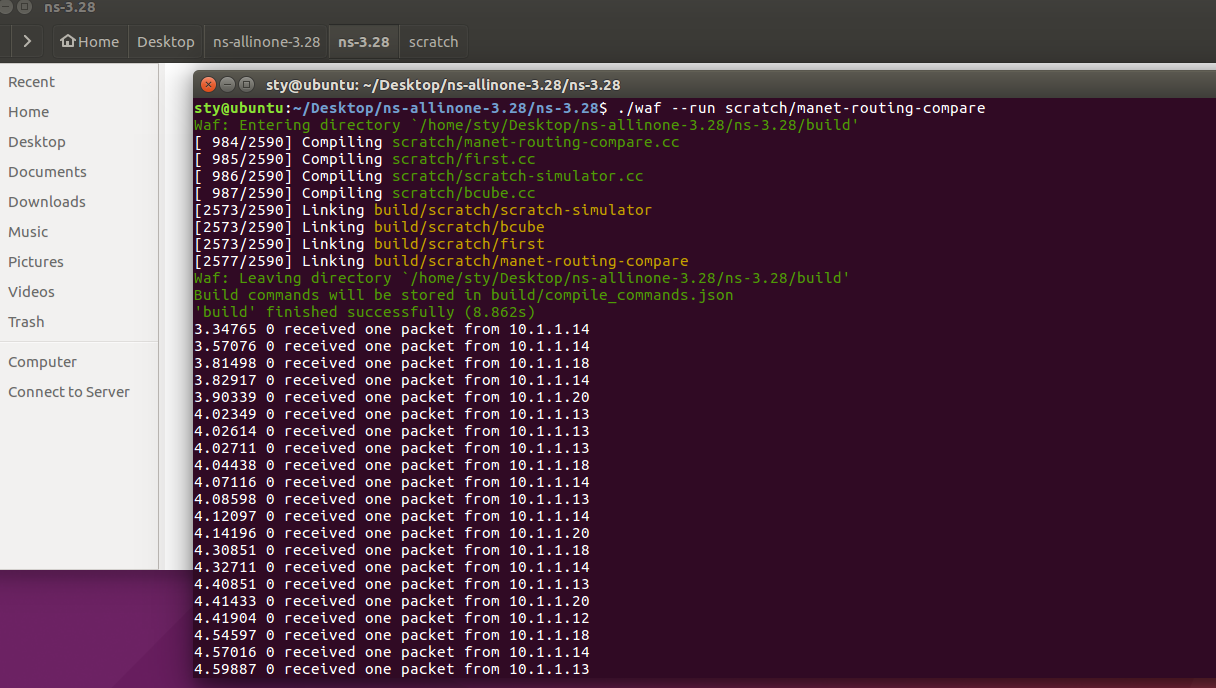
\includegraphics[width=0.8\linewidth]{image/screenshot021}
	\caption{编译并运行manet-routing.cc}
	\label{fig:screenshot021}
\end{figure}


3、显示运行动画

1)将目录移动到执行目录netanim

2)启动netanim动画工具程序:./NetAnim

3)显示运行动画。打开manet-routing.xml

\begin{figure}[htbp]
	\centering
	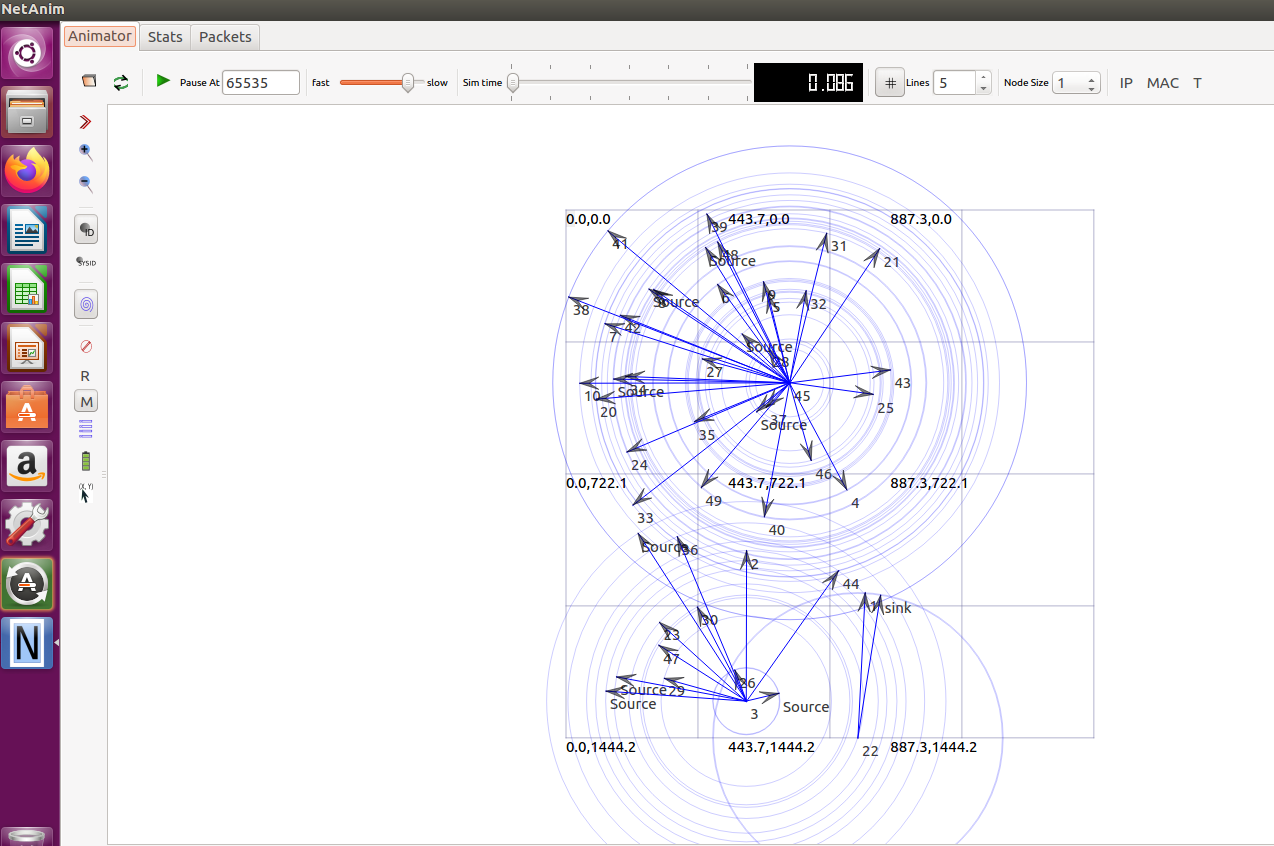
\includegraphics[width=0.9\linewidth]{image/screenshot022}
	\caption{显示运行动画}
	\label{fig:screenshot022}
\end{figure}


【实验小结】

无线自组织网络有非常多的应用情形,这个简单的,非常经典的demo带我入门,领略了ns3的强大之处。

\subsection{实验小结}

通过本次虚拟无线网络实验,初步了解了ns3的使用方法和它的强大之处,也为后续做NS3自选实验做好了铺垫。

第二个实验我特别关注了,在现实中,有很多关于无线自组织网络的研究,例如在本次的自选实验中,我们曾关注过一篇车用自组织网络(VANETs),其中详细介绍了车用自组织网络的工作方法,还基于NS3研究了车用自组织网络的路由协议的性能。较之一般的Ad hoc网络,VANETs的动态特性更为明显。VANETs当中的汽车节点移动速度更快、拓扑变化更频繁、路径寿命更短。同时,VANETs当中的汽车节点移动模型比较复杂,车辆节点密度不均匀等特点也给VANETs的研究工作带来了极大的困难。

\section{静态路由配置实验}
\subsection{实验目的}

静态路由,是指由人工根据网络拓扑结构来创建路由表。路由器需要依靠路由表来转发 IP数据包,该实验是路由器实验中最基础的实验,后续的几个实验都以静态路由为基础。静态路由也是理解路由原理最直观的途径。实验模仿两个远程子网的互联,两个子网在本地各 接一个路由器,路由器之间用远程网络相连,使用静态路由实现远程子网互联。

(1)	深入了解IP路由基本原理。

(2)	了解和掌握配置静态路由配置方法。

\subsection{实验设备}

实验环境由两台路由器、两台计算机和一台交换机组成,模拟两个远程子网互联。使用单根串行交叉线将两个路由器的串口对接起来,代表路由器之间的远程网络;将路由器以太网端口和两台计算机网卡都用网线直接连接到交换机,由交换机担当网络连接;通过串行线将计算机串口com同路由器console口连接起来,两台计算机超级终端将作为路由器管理的操作平台。

\subsection{实验网络拓扑}


\begin{figure}[htbp]
	\centering
	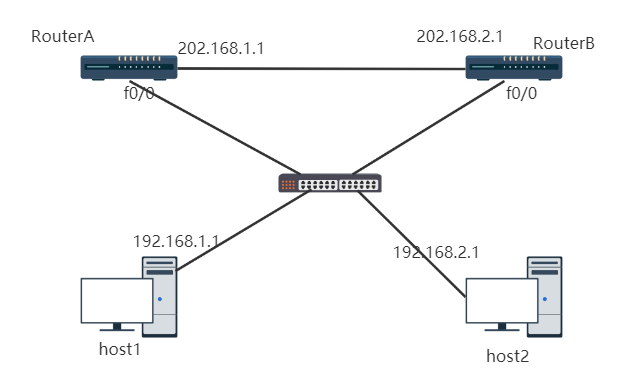
\includegraphics[width=0.7\linewidth]{image/screenshot024}
	\caption{静态路由实验实验网络拓扑}
	\label{fig:screenshot024}
\end{figure}


\subsection{实验内容}

\begin{lstlisting}
1.连接路由器
--打开路由器电源
--使用console线将计算机串口com1与路由器console口直接相连;
--建立HyperTerminal:开始程序附件通讯超级终端名称=router连接=com1Baut Rate=9600,8,no parity, 1 stop bit;
--进入特权模式:router01>en(able) ,Enable Secret Password=cisco
2查看端口状态:
--记录以太0/0口IP地址:router01# sh interface g 0/0
--记录串口0/0口IP地址:router01# sh interface ser 0/0/1
3配置快速以太f0/0
--进入配置模式:router01#config t
--进入以太口:router01(config)#in g0/0
--删除旧IP地址: router01(config-if)#no ip address <ipaddress><subnet mask>
--添加IP地址: router01(config-if)#ip address <ipaddress><subnet mask>
--开启端口功能:router01(config-if)#no shut
4配置串口s0/0
--退到配置模式:router01(config-if)#exit
--进入串口:router01(config)#in s0/0/1
--设置新IP地址
5 静态路由
5.1添加对端路由: router01(config)#ip route 192.168.y.0 255.255.255.0 202.168.1.z # 对端网络地址和广域端口地址;
5.2查看路由表:  router01# sh ip route
5.3 打开路由功能:router01# config t
router01(config)#ip routing
router01(config-if)#exit
5.4 测试
--配置计算机IP地址:192.168.x.254
--测试连通(从计算机):ping 192.168.y.254# 对端计算机
6 缺省路由
6.1删除静态路由: router01(config)#no ip route 192.168.y.0 255.255.255.0 
6.2添加缺省路由: router01(config)#ip route 0.0.0.0 0.0.0.0 202.168.1.z # 对端网络地址和广域端口地址;
6.3查看路由表:router01# sh ip route
6.4 测试
--测试连通(从计算机):ping 192.168.y.254# 对端计算机
7查看运行配置:router01# sh running config

\end{lstlisting}


\begin{figure}[htbp]
	\centering
	\includegraphics[width=0.7\linewidth]{image/1907846D1B5FCD168DC34B37C57127CE}
	\caption{用 sh ip route 查看路由表的照片}
	\label{fig:1907846d1b5fcd168dc34b37c57127ce}
\end{figure}


\begin{figure}[htbp]
	\centering
	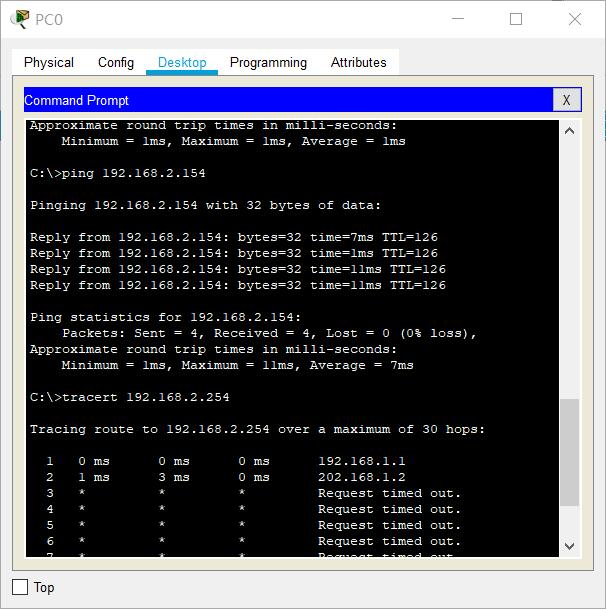
\includegraphics[width=0.7\linewidth]{image/QQ截图20201028235123}
	\caption{用tracert 跟踪路径}
	\label{fig:qq20201028235123}
\end{figure}

\begin{figure}[htbp]
	\centering
	\includegraphics[width=0.7\linewidth]{image/E7210D63DB010B2DDCD3092AFB1AB061}
	\caption{静态路由配置成功,ping通了的照片}
	\label{fig:e7210d63db010b2ddcd3092afb1ab061}
\end{figure}


\subsection{实验小结}

本次实验还是遇到了不少小问题的,在金老师的指导下也收获了不少debug的方法。

1.计网实验教室系统重装过了,防火墙没关,导致一开始ping不通。

2.一开始完成实验操作后并没有ping通两台主机,经过排查,查看路由器路由表的时候发现没有从路由器1到路由器2的路由,但是这个路由应该已经在之前的操作里设置过了,据此断定是因为串口接触不良,串口接触良好后再次查看路由器的路由表,对应的路由就出现了。

3.\textbf{配置时和已有的路由冲突了,使用no命令删除了冲突的IP,最后配置成功。这点很重要!}当时因为冲突报错困扰了我很长时间。

4.许多串口可能接触不良,最后我总结出经验,需要使用no shut命令配合串口旁边的指示灯来判断串口是否正常。

5.接线前先检查包括串口在内的各部件是否工作正常,正常后再进行进一步的实验,以免实验失败了还难以排查问题。

\section{RIP动态路由实验}
\subsection{实验目的}

1.	了解和掌握路由信息协议 RIP 概念;

2.	配置 RIP 动态路由,实现网际通信。

这一讲书上没有写,只能看文档了。

\subsection{实验设备}

两台路由器,使用串行线将两个 0 串口对接;两台计算机作为操作平台;一台交换机担当网络连接。

\subsection{实验网络拓扑}
实验网络拓扑和静态路由是一样的,只不过路由表不用自己设置了。

\begin{figure}[htbp]
	\centering
	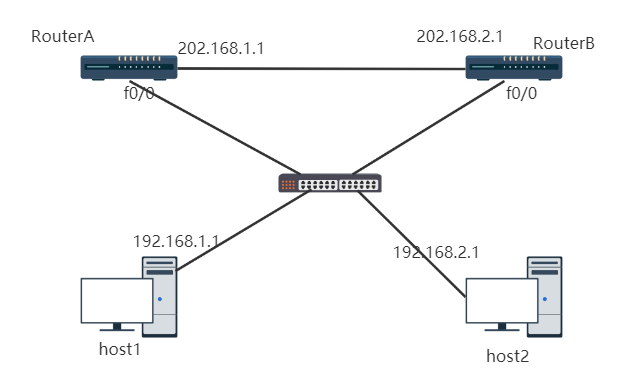
\includegraphics[width=0.7\linewidth]{image/screenshot024}
	\caption{RIP动态路由实验实验网络拓扑}
	\label{fig:screenshot024-2}
\end{figure}

\subsection{实验内容}

\begin{lstlisting}
连接路由器
--打开路由器电源
--使用console线将计算机串口com1与路由器console口直接相连;
--建立HyperTerminal:开始程序附件通讯超级终端名称=router连接=com1Baut Rate=9600,8,no parity, 1 stop bit;
--进入特权模式:router01>en(able) ,Enable Secret Password=cisco
2查看端口状态:router01# sh interface
记录IP地址;
3配置快速以太网f0/0
--进入配置模式:router01#config t
--进入以太口:router01(config)#in f0/0
--删除旧IP地址: router01(config-if)#no ip address <ipaddress><subnet mask>
--添加IP地址: router01(config-if)#ip address <ipaddress><subnet mask>
--开启端口功能:router01(config-if)#no shut
4配置串口s0/0
--退到配置模式:router01(config-if)#exit
--进入串口:router01(config)#in s0/0
--设置IP地址: router01(config-if)#ip addr 202.168.1.1 255.255.255.0
5配置串口s0/1
--退到配置模式:router01(config-if)#exit
--进入串口:router01(config)#in s0/1
--设置IP地址: router01(config-if)#ip addr 202.168.2.1 255.255.255.0
--设置带宽: router01(config-if)#band 256
6 配置RIP动态路由
--添加RIP: router01(config)#router rip #如果路由功能关闭,rip必须重新配置;
--指定邻居网络:router01(config-router)# network 192.168.1.0
router01(config-router)# network 202.168.1.0
router01(config-router)# network 202.168.2.0
--查看RIP路由表:router01# sh ip route rip 
7 测试
--配置计算机IP地址:192.168.x.254
-- router01#no ip domain-lookup
-- router01#trace ip 192.168.2.250
8 跟踪调试
-- router01#debug ip rip#查看信息发送端口
9 被动接口设置 
--进入RIP设置: router01(config)#router rip
--以太网端口配置成被动模式: router01(config-router)#passive-interface f0/0
--查看调试:以太口不再发送

\end{lstlisting}

实验拍照如下图\ref{fig:63f1c6dd39df7a536df3207bdc2cd44}:


\begin{figure}[htbp]
	\centering
	\includegraphics[width=0.7\linewidth]{image/63f1c6dd39df7a536df3207bdc2cd44}
	\caption{RIP动态路由实验截图}
	\label{fig:63f1c6dd39df7a536df3207bdc2cd44}
\end{figure}



\subsection{实验小结}

本次动态路由实验也遇到了一定的问题,在第一次尝试中遇到了线路无法接通的困惑,具体如下:在配置完所有端口后,在两个路由器的四个串口上的指示灯只亮了三展,在router1的s0/0/0口上指示灯是亮的,而在router2的s0/0/0口上指示灯是灭的,并且并不是指示灯坏了,指示灯有时是能断续发一点光的。

实验结果是,利用tracert查看路由,发现包通过了s0/0/1口,也就是限速的串口,并且延迟很高(大约20ms),这说明串口配置确实有问题,这令人百思不得其解。

同时,在计算机网络课程的学习中,我得知了RIP是距离向量路由算法(DVR 计算机网络与因特网第六版P203)的实现,OSPF是链路状态路由协议(LSR 计算机网络与因特网第六版P202)的实现,这让我对动态路由算法的底层原理有了更深入的了解。

\section{OSPF动态路由实验}
\subsection{实验目的}

动态路由是指由软件根据网络拓扑结构自动构建路由表,适合于较大规模网络的路由配置。最难能可贵的是动态路由能自动适应网络故障,一旦发生网络故障,会根据网络故障发生 情况重新生成路由表,及时消除故障的影响。动态路由配置技能是路由器管理的主要工程技能,必须熟悉和掌握。实验模仿两个远程子网的互联,两个子网各接一个路由器,路由器之间用远程网络相连,使用开放式最短路径优先协议(OSPF)实现远程子网互联。

(1)	了解动态路由表生成基本原理。

(2)	了解最短路径优先算法基本思想。

(3)	了解掌握OSPF动态路由技能。


\subsection{实验设备}

实验环境主要由两台路由器、两台计算机和一台交换机组成。使用两根串行交叉线将两个路由器的串口对接起来,创建两个远程传输子网,便于动态路由选择;将路由器以太网端口 和两台计算机网卡都用网线直接连接交换机,由交换机担当网络连接;通过串行线将计算机串口com同路由器console口连接起来,两台计算机超级终端作为路由器管理的操作平台。

\subsection{实验网络拓扑}

实验网络拓扑还是和静态路由是一样的,只不过路由表不用自己设置了。如图\ref{fig:screenshot024-3}所示。

\begin{figure}[htbp]
	\centering
	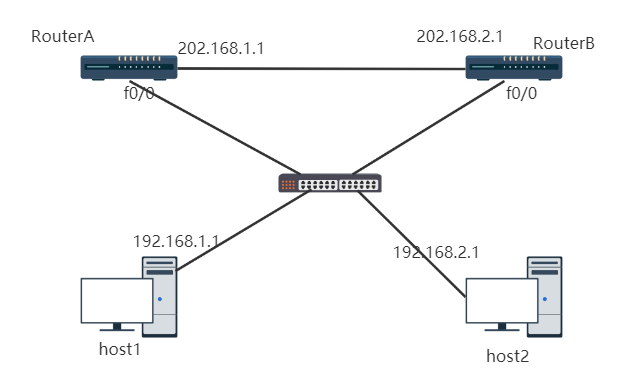
\includegraphics[width=0.7\linewidth]{image/screenshot024}
	\caption{OSPF动态路由实验实验网络拓扑}
	\label{fig:screenshot024-3}
\end{figure}


\subsection{实验内容}

\begin{lstlisting}
连接路由器
--打开路由器电源
--使用console线将计算机串口com1与路由器console口直接相连;
--建立HyperTerminal:开始程序附件通讯超级终端名称=router连接=com1Baut Rate=9600,8,no parity, 1 stop bit;
--进入特权模式:router01>en(able) ,Enable Secret Password=cisco
2查看端口状态:router01# sh interface
记录IP地址;
3配置快速以太网f0/0
--进入配置模式:router01#config t
--进入以太口:router01(config)#in f0/0
--删除旧IP地址: router01(config-if)#no ip address <ipaddress><subnet mask>
--添加IP地址: router01(config-if)#ip address <ipaddress><subnet mask>
--开启端口功能:router01(config-if)#no shut
4配置串口s0/0
--退到配置模式:router01(config-if)#exit
--进入串口:router01(config)#in s0/0
--设置IP地址: router01(config-if)#ip addr 202.168.1.1 255.255.255.0
5配置串口s0/1
--退到配置模式:router01(config-if)#exit
--进入串口:router01(config)#in s0/1
--设置IP地址: router01(config-if)#ip addr 202.168.2.1 255.255.255.0
--设置带宽: router01(config-if)#band 256
6 配置OSPF动态路由
--添加OSPF: router01(config)#router ospf 100 #如果路由功能关闭,rip必须重新配置;
--指定邻居网络:router01(config-router)# network 192.168.1.0 0.0.0.255 area 0
router01(config-router)# network 202.168.1.0 0.0.0.255 area 0
router01(config-router)# network 202.168.2.0 0.0.0.255 area 0
--查看OSPF ID:router01# sh ip ospf int 
--查看OSPF路由表:router01# sh ip route ospf 
--查看OSPF邻居:router01# sh ip ospf nei
7 测试
--配置计算机IP地址:192.168.x.254
-- router01#no ip domain-lookup
-- router01#trace ip 192.168.2.250
8 跟踪调试
-- router01#debug ip ospf#查看信息发送端口

\end{lstlisting}

\begin{figure}[htbp]
	\centering
	\includegraphics[width=0.7\linewidth]{image/4035bc3b7ac7d1a0c09d9908097465f}
	\caption{OSPF实验拍照}
	\label{fig:4035bc3b7ac7d1a0c09d9908097465f}
\end{figure}


\subsection{实验小结}

本次的实验是和RIP路由一起做的。

在第一次尝试中遇到了线路无法接通的困惑,具体如下:在配置完所有端口后,在两个路由器的四个串口上的指示灯只亮了三展,在router1的s0/0/0口上指示灯是亮的,而在router2的s0/0/0口上指示灯是灭的,并且并不是指示灯坏了,指示灯有时是能断续发一点光的。
实验结果是,利用tracert查看路由,发现包通过了s0/0/1口,也就是限速的串口,并且延迟很高(大约20ms),这说明串口配置确实有问题,这令人百思不得其解。

同时,在计算机网络课程的学习中,我得知了RIP是距离向量路由算法(DVR 计算机网络与因特网第六版P203)的实现,OSPF是链路状态路由协议(LSR 计算机网络与因特网第六版P202)的实现,这让我对动态路由算法的底层原理有了更深入的了解。

\section{帧中继配置实验}
\subsection{实验目的}

广域网是另一类主要有线物理网络,可以实现跨地域的网络连接,承担着骨干传输网络作用,只有ISP(Internet Service Provider,互联网服务提供商)才会拥有,如中国电信、移动等,普通企业很难见到此类设备。因此本书没有对广域网进行详尽介绍,但了解广域网网络和局域网互联,有助于深入理解网际网的异构特性。本实验利用路由器模拟帧中继交换机,用于远程连接两个以太网,实现网络互联。

(1)	了解广域网基本概念。

(2)	区分二层路由和三层路由基本概念。

(3)	熟悉帧中继交换机永久虚电路及配置步骤。

\subsection{实验设备}

实验环境主要由三台路由器、三台计算机和一台交换机组成,模拟一个由局域网和广域网组成的网际网。路由器(模拟帧中继交换机)使用单根串行交叉线将路由器A和路由器C的 广域网串口连接起来,路由器B和路由器C的广域网串口连接起来(构建帧中继网络专线以连接两个远程子网),并使得同RouterC相连的电缆连接线类型均为DCE,将路由器A和路由 器B以太网端口和两台计算机网卡都用网线直接连接到交换机,由交换机担当网络连接;通过串行线将各个计算机串口com同路由器console口连接起来,使用各自超级终端作为路由器管理的操作平台。

\subsection{实验网络拓扑}



\subsection{实验内容}
\subsection{实验小结}
\section{组播实验}
\subsection{实验目的}
\subsection{实验设备}
\subsection{实验网络拓扑}
\subsection{实验内容}
\subsection{实验小结}
\section{动态IP地址分配DHCP实验}
\subsection{实验目的}
\subsection{实验设备}
\subsection{实验网络拓扑}
\subsection{实验内容}
\subsection{实验小结}
\section{ACL访问控制实验}
\subsection{实验目的}
\subsection{实验设备}
\subsection{实验网络拓扑}
\subsection{实验内容}
\subsection{实验小结}
\section{邮件收发实验}
\subsection{实验目的}
\subsection{实验设备}
\subsection{实验网络拓扑}
\subsection{实验内容}
\subsection{实验小结}
\section{ARP消息分析实验}
\subsection{实验目的}
\subsection{实验设备}
\subsection{实验网络拓扑}
\subsection{实验内容}
\subsection{实验小结}
\section{IP数据包分析实验}
\subsection{实验目的}
\subsection{实验设备}
\subsection{实验网络拓扑}
\subsection{实验内容}
\subsection{实验小结}
\section{UDP用户数据报分析实验}
\subsection{实验目的}
\subsection{实验设备}
\subsection{实验网络拓扑}
\subsection{实验内容}
\subsection{实验小结}
\section{NAT网络地址转换实验}
\subsection{实验目的}
\subsection{实验设备}
\subsection{实验网络拓扑}
\subsection{实验内容}
\subsection{实验小结}
\section{个人文献阅读}
\section{自选型综合实验}
\subsection{实验目的}
\subsection{实验设备}
\subsection{实验网络拓扑}
\subsection{实验内容}
\subsection{实验小结}

\subsection{模板介绍}

此模板基于 \LaTeX{} 的标准文类 article 设计,所以 article 文类的选项也能传递给本模板,比如 \lstinline{a4paper, 11pt} 等等。本模板支持 \hologo{pdfLaTeX} 和 \hologo{XeLaTeX} 编译。

\begin{lstlisting}
\documentclass[a4paper,11pt]{elegantpaper}
\end{lstlisting}

\textbf{注意}:Elegant\LaTeX{} 系列模板已经全部上传至 \href{https://www.overleaf.com/latex/templates/elegantpaper-template/yzghrqjhmmmr}{Overleaf} 上,用户可以在线使用。另外,为了方便国内用户,模板也已经传至\href{https://gitee.com/ElegantLaTeX/ElegantPaper}{码云}。


\subsection{全局选项}
此模板定义了一个语言选项 \lstinline{lang},可以选择英文模式 \lstinline{lang=en}(默认)或者中文模式 \lstinline{lang=cn}。当选择中文模式时,图表的标题引导词以及参考文献,定理引导词等信息会变成中文。你可以通过下面两种方式来选择语言模式:
\begin{lstlisting}
\documentclass[lang=cn]{elegantpaper} % or
\documentclass{cn}{elegantpaper} 
\end{lstlisting}

\textbf{注意:} 英文模式下,由于没有添加中文宏包,无法输入中文。如果需要输入中文,可以通过在导言区引入中文宏包 \lstinline{ctex} 或者加入 \lstinline{xeCJK} 宏包后自行设置字体。 
\begin{lstlisting}
\usepackage[UTF8,scheme=plain]{ctex}
\end{lstlisting}

\subsection{数学字体选项}

本模板定义了一个数学字体选项(\lstinline{math}),可选项有三个:
\begin{enumerate}
  \item \lstinline{math=cm}(默认),使用 \LaTeX{} 默认数学字体(推荐,无需声明);
  \item \lstinline{math=newtx},使用 \lstinline{newtxmath} 设置数学字体(潜在问题比较多)。
  \item \lstinline{math=mtpro2},使用 \lstinline{mtpro2} 宏包设置数学字体,要求用户已经成功安装此宏包。
\end{enumerate}

\subsection{中文字体选项}
模板提供中文字体选项 \lstinline{chinesefont},可选项有
\begin{enumerate}
\item \lstinline{ctexfont}:默认选项,使用 \lstinline{ctex} 宏包根据系统自行选择字体,可能存在字体缺失的问题,更多内容参考 \lstinline{ctex} 宏包\href{https://ctan.org/pkg/ctex}{官方文档}\footnote{可以使用命令提示符,输入 \lstinline{texdoc ctex} 调出本地 \lstinline{ctex} 宏包文档}。
\item \lstinline{founder}:方正字体选项,调用 \lstinline{ctex} 宏包并且使用 \lstinline{fontset=none} 选项,然后设置字体为方正四款免费字体,方正字体下载注意事项见后文。
\item \lstinline{nofont}:调用 \lstinline{ctex} 宏包并且使用 \lstinline{fontset=none} 选项,不设定中文字体,用户可以自行设置中文字体,具体见后文。
\end{enumerate}

\noindent \textbf{注意:} 使用 \lstinline{founder} 选项或者 \lstinline{nofont} 时,必须使用 \hologo{XeLaTeX} 进行编译。

\subsubsection{方正字体选项}
由于使用 \lstinline{ctex} 宏包默认调用系统已有的字体,部分系统字体缺失严重,因此,用户希望能够使用其它字体,我们推荐使用方正字体。方正的{\songti 方正书宋}、{\heiti 方正黑体}、{\kaishu 方正楷体}、{\fangsong 方正仿宋}四款字体均可免费试用,且可用于商业用途。用户可以自行从\href{http://www.foundertype.com/}{方正字体官网}下载此四款字体,在下载的时候请\textbf{务必}注意选择 GBK 字符集,也可以使用 \href{https://www.latexstudio.net/}{\LaTeX{} 工作室}提供的\href{https://pan.baidu.com/s/1BgbQM7LoinY7m8yeP25Y7Q}{方正字体,提取码为:njy9} 进行安装。安装时,{\kaishu Win 10 用户请右键选择为全部用户安装,否则会找不到字体。}

\begin{figure}[!htb]
\centering

\end{figure}

\subsubsection{其他中文字体}
如果你想完全自定义字体\footnote{这里仍然以方正字体为例。},你可以选择 \lstinline{chinesefont=nofont},然后在导言区设置
\begin{lstlisting}
\setCJKmainfont[BoldFont={FZHei-B01},ItalicFont={FZKai-Z03}]{FZShuSong-Z01}
\setCJKsansfont[BoldFont={FZHei-B01},ItalicFont={FZHei-B01}]{FZHei-B01}
\setCJKmonofont[BoldFont={FZHei-B01},ItalicFont={FZHei-B01}]{FZFangSong-Z02}
\setCJKfamilyfont{zhsong}{FZShuSong-Z01}
\setCJKfamilyfont{zhhei}{FZHei-B01}
\setCJKfamilyfont{zhkai}{FZKai-Z03}
\setCJKfamilyfont{zhfs}{FZFangSong-Z02}
\newcommand*{\songti}{\CJKfamily{zhsong}}
\newcommand*{\heiti}{\CJKfamily{zhhei}}
\newcommand*{\kaishu}{\CJKfamily{zhkai}}
\newcommand*{\fangsong}{\CJKfamily{zhfs}}
\end{lstlisting}


\subsection{自定义命令}
此模板并没有修改任何默认的 \LaTeX{} 命令或者环境\footnote{目的是保证代码的可复用性,请用户关注内容,不要太在意格式,这才是本工作论文模板的意义。}。另外,我自定义了 4 个命令:
\begin{enumerate}
  \item \lstinline{\email}:创建邮箱地址的链接,比如 \email{ddswhu@outlook.com};
  \item \lstinline{\figref}:用法和 \lstinline{\ref} 类似,但是会在插图的标题前添加 <\textbf{图 n}> ;
  \item \lstinline{\tabref}:用法和 \lstinline{\ref} 类似,但是会在表格的标题前添加 <\textbf{表 n}>;
  \item \lstinline{\keywords}:为摘要环境添加关键词。
\end{enumerate}

\subsection{参考文献}
此模板使用 \hologo{BibTeX} 来生成参考文献,中文模式下默认使用的文献样式(bib style)是 \lstinline{GB/T 7714-2015}\footnote{通过调用 \href{https://ctan.org/pkg/gbt7714}{\lstinline{gbt7714}} 宏包}。参考文献示例:~\cite{en3} 使用了中国一个大型的 P2P 平台(人人贷)的数据来检验男性投资者和女性投资者在投资表现上是否有显著差异。

你可以在谷歌学术,Mendeley,Endnote 中获得文献条目(bib item),然后把它们添加到 \lstinline{wpref.bib} 中。在文中引用的时候,引用它们的键值(bib key)即可。注意需要在编译的过程中添加 \hologo{BibTeX} 编译。

本模板还添加了 \lstinline{cite=numbers} 、\lstinline{cite=super} 和 \lstinline{cite=authoryear}  三个参考文献选项,用于设置参考文献格式的设置,默认为 \lstinline{numbers}。理工科类一般使用数字形式 \lstinline{numbers} 或者上标形式 \lstinline{super},而文科类多使用作者-年份 \lstinline{authoryear} 比较多。如果需要改为 \lstinline{cite=numbers}  或者  \lstinline{authoryear} ,可以使用
\begin{lstlisting}
\documentclass[cite=super]{elegantpaper} % super style ref style
\documentclass[super]{elegantpaper}

\documentclass[cite=authoryear]{elegantpaper} % author-year ref style
\documentclass[authoryear]{elegantpaper}
\end{lstlisting}


\section{协作人员招募}
招募 Elegant\LaTeX{} 的协作人员,没有工资。工作内容:翻译 Elegant\LaTeX{} 系列模板相关的文稿(中翻英),维护模板的 wiki(主要涉及 Markdown),如果有公众号文稿写作经历的话,也可以帮忙写微信稿。本公告长期有效。

目前 ElegantLaTeX 共有 4 名协作人员,分别是
\begin{itemize}
  \item 官方文档翻译: \href{https://github.com/peggy2006xzyz}{YPY};
  \item GitHub 维基维护: \href{https://github.com/izinngo}{Ingo Zinngo}、\href{https://github.com/xiaohao890809}{追寻原风景};
  \item QQ 群管理员: \href{https://github.com/sikouhjw}{Sikouhjw}.
\end{itemize}

在此感谢他们无私的奉献!


\section{致谢}
截止到 2020 年 04 月 12 日,ElegantPaper v0.09 版本发布,ElegantPaper 模板在 GitHub 上的收藏数(star)达到了 277。在此特别感谢 China\TeX{} 以及 \href{http://www.latexstudio.net/}{\LaTeX{} 工作室}对于本系列模板的大力宣传与推广。如果你喜欢我们的模板,你可以在 GitHub 上收藏(Star)我们的模板。
\begin{figure}[htbp]
  \centering

  \caption{一键三连求赞}
\end{figure}

\section{捐赠}
如果您非常喜爱我们的模板,你还可以选择捐赠以表达您对我们模板和我的支持!

\begin{figure}[htbp]
  \centering

\end{figure}

\textbf{赞赏费用的使用解释权归 Elegant\LaTeX{} 所有,并且不接受监督,请自愿理性打赏}。10 元以上的赞赏,我们将列入捐赠榜,谢谢各位金主!


\begin{table}[!htb]
  \centering
  \caption{Elegant\LaTeX{} 系列模板捐赠榜}
    \begin{tabular}{*{4}{>{\scriptsize}c}|*{4}{>{\scriptsize}c}}
    \hline
    \textbf{捐赠者} & \textbf{金额} & \textbf{时间} & \textbf{渠道} & \textbf{捐赠者} & \textbf{金额} & \textbf{时间} & \textbf{渠道} \\
    \hline
    Lerh  & 10 RMB & 2019/05/15 & 微信    & 越过地平线 & 10 RMB & 2019/05/15 & 微信 \\
    银桑    & 20 RMB & 2019/05/27 & 微信    & *空    & 10 RMB & 2019/05/30 & 微信 \\
    latexstudio.net & 666 RMB & 2019/06/05 & 支付宝   & A*n   & 40 RMB & 2019/06/15 & 微信 \\
    * 夏   & 22 RMB & 2019/06/15 & 微信    & * 倩   & 21 RMB  & 2019/06/15 & 微信 \\
    Cassis & 11 RMB & 2019/06/30 & 微信    & *君    & 10 RMB & 2019/07/23 & 微信 \\
    P*u   & 50 RMB & 2019/07/30 & 微信    & *萌    & 19 RMB & 2019/08/28 & 微信 \\
    曲豆豆   & 10 RMB & 2019/08/28 & 微信    & 李博    & 100 RMB & 2019/10/06 & 微信 \\
    Njustsll & 10 RMB & 2019/10/11 & 微信    & 刘志阔   & 99.99 RMB & 2019/10/15 & 支付宝 \\
    * 韬   & 16 RMB & 2019/10/17 & 微信    & 赤霓    & 12 RMB & 2019/10/17 & 支付宝 \\
    追寻原风景 & 10 RMB & 2019/10/28 & 微信    & 郭德良   & 88 RMB & 2019/11/03 & 微信 \\
    自强不息  & 20 RMB & 2019/11/04 & 支付宝   & 读书之虫  & 20 RMB & 2019/11/18 & 微信 \\
    *等    & 10 RMB & 2019/11/18 & 微信    & *哲    & 20 RMB & 2019/11/18 & 微信 \\
    佚名    & 10 RMB & 2019/11/24 & 微信    & Jiye Qian & 66 RMB & 2019/12/04 & 微信 \\
    * 阳   & 20 RMB & 2019/12/05 & 微信    & Catcher & 11 RMB & 2019/12/08 & 支付宝 \\
    希尔波特门徒 & 10 RMB & 2019/12/09 & 支付宝   & * 伟   & 10 RMB & 2019/12/09 & 微信 \\
    Simon & 20 RMB & 2019/12/11 & 支付宝   & 流殇丶浅忆 & 66.60 RMB & 2019/12/18 & 支付宝 \\
    羽     & 10 RMB & 2019/12/20 & 支付宝   & * 琛   & 15 RMB & 2019/12/20 & 微信 \\
    随风    & 20 RMB & 2019/12/27 & 支付宝   & Ws    & 23.30 RMB & 2019/12/28 & 微信 \\
    初八    & 100 RMB  & 2020/01/02 & 支付宝   & p*e   & 20 RMB & 2020/01/03 & 微信 \\
    Shunmx & 100 RMB & 2020/01/03 & 微信    & hj    & 10 RMB & 2020/01/03 & 微信 \\
    F*5   & 10 RMB & 2020/01/03 & 微信    & S*m   & 20.20 RMB & 2020/01/03 & 微信 \\
    二代青雉  & 13 RMB & 2020/01/14 & 支付宝   & *?    & 66 RMB & 2020/01/15 & 微信 \\
    Mr. Xiong & 20 RMB & 2020/01/17 & 微信    & *博    & 15 RMB & 2020/01/18 & 微信 \\
    * 者  & 10 RMB & 2020/02/02 & 微信    & Jackie  &  88.80 RMB  &  2020/02/09 & 微信 \\
    Henry\_Sun、 & 50 RMB & 2020/02/14 & 支付宝 & * 桥  & 50 RMB & 2020/02/21 & 微信 \\
    昀琏 & 10 RMB & 2020/03/02 & 支付宝 & S*y  &  10 RMB  &  2020/03/15 & 微信 \\
    * 哥  & 66.66 RMB & 2020/03/17 & 微信    &   K*e & 30 RMB & 2020/03/30 & 微信\\
    * 阳  &  20 RMB  &  2020/04/02 & 微信 & 士*n  & 30 RMB & 2020/04/11 & 微信 \\
    \hline
    \end{tabular}%
  \label{tab:donation}%
\end{table}%

\section{常见问题 FAQ}

\begin{enumerate}[label=\arabic*).]
  \item \textit{如何删除版本信息?}\\
      导言区不写 \lstinline|\version{x.xx}| 即可。
  \item \textit{如何删除日期?}\\
      需要注意的是,与版本 \lstinline{\version} 不同的是,导言区不写或注释 \lstinline{\date} 的话,仍然会打印出当日日期,原因是 \lstinline{\date} 有默认参数。如果不需要日期的话,日期可以留空即可,也即 \lstinline|\date{}|。
  \item \textit{如何获得中文日期?}\\
      为了获得中文日期,必须在中文模式下\footnote{英文模式下,由于未加载中文宏包,无法输入中文。},使用 \lstinline|\date{\zhdate{2019/10/11}}|,如果需要当天的汉化日期,可以使用 \lstinline|\date{\zhtoday}|,这两个命令都来源于 \href{https://ctan.org/pkg/zhnumber}{\lstinline{zhnumber}} 宏包。
  \item \textit{如何添加多个作者?}\\
      在 \lstinline{\author} 里面使用 \lstinline{\and},作者单位可以用 \lstinline{\\} 换行。\begin{lstlisting}
\author{author 1\\ org. 1 \and author 2 \\ org. 2 }
\end{lstlisting}
  \item \textit{如何添加中英文摘要?}\\
      请参考 \href{https://github.com/ElegantLaTeX/ElegantPaper/issues/5}{GitHub::ElegantPaper/issues/5}
\end{enumerate}

\section{示例}

为了让大家更加清楚最终的论文效果,如下给出两篇使用 ElegantPaper 模板排版的工作论文示例,也欢迎大家"投稿"!

\begin{enumerate}
  \item \href{https://github.com/EthanDeng/bank-custody}{银行存管、投资者决策与 P2P 网络借贷规范发展};
  \item \href{https://github.com/EthanDeng/risk-awareness}{互联网金融风险与投资者风险意识 —— 来自网贷平台交易数据的证据}。
\end{enumerate}


\nocite{*}
\bibliography{wpref}

\appendix
%\appendixpage
\addappheadtotoc
\section{使用 newtx 系列字体}

如果需要使用原先版本的 \lstinline{newtx} 系列字体,可以通过显示声明数学字体:

\begin{lstlisting}
\documentclass[math=newtx]{elegantbook}
\end{lstlisting}

\subsection{连字符}

如果使用 \lstinline{newtx} 系列字体宏包,需要注意下连字符的问题。
\begin{equation}
  \int_{R^q} f(x,y) dy.\emph{of\kern0pt f}
\end{equation}
的代码为
\begin{lstlisting}
\begin{equation}
  \int_{R^q} f(x,y) dy.\emph{of \kern0pt f}
\end{equation}
\end{lstlisting}

\subsection{宏包冲突}

另外在 ElegantBook 模板中,有用户反馈模板在使用 \lstinline{yhmath} 以及 \lstinline{esvect} 等宏包时会报错:
\begin{lstlisting}
LaTeX Error:
   Too many symbol fonts declared.
\end{lstlisting}

原因是在使用 \lstinline{newtxmath} 宏包时,重新定义了数学字体用于大型操作符,达到了 {\heiti 最多 16 个数学字体} 的上限,在调用其他宏包的时候,无法新增数学字体。为了减少调用非常用宏包,在此给出如何调用 \lstinline{yhmath} 以及 \lstinline{esvect} 宏包的方法。

请在 \lstinline{elegantpaper.cls} 内搜索 \lstinline{yhmath} 或者 \lstinline{esvect},将你所需要的宏包加载语句\textit{取消注释}即可。
\begin{lstlisting}
%%% use yhmath pkg, uncomment following code
% \let\oldwidering\widering
% \let\widering\undefined
% \RequirePackage{yhmath}
% \let\widering\oldwidering

%%% use esvect pkg, uncomment following code
% \RequirePackage{esvect}
\end{lstlisting}


\end{document}
